\documentclass[11pt]{article}
\usepackage[a4paper,margin=1in]{geometry}
\usepackage{graphicx}
\usepackage{booktabs}
\usepackage{array}
\usepackage{amsmath}
\usepackage{caption}
\usepackage{float}
\usepackage[super,numbers,sort&compress]{natbib}
\usepackage{enumitem}
\usepackage{anyfontsize}
\usepackage{xeCJK}
\setCJKmainfont[BoldFont=SimHei]{SimSun}
\newCJKfontfamily\heiti{SimHei}[AutoFakeBold=2.2]
\usepackage{tikz}
\usepackage[hidelinks]{hyperref}
\Urlmuskip=0mu plus 1mu\relax
\setlength{\emergencystretch}{2em}
\hyphenation{comparables comparable}% never hyphenate "comparable(s)" across a line break
\graphicspath{{../figures/}{./}}
\captionsetup{font=small,labelfont=bf}
\setlength{\parskip}{0.4em}
\setlength{\parindent}{0pt}

\newcommand{\papertitle}{Capability Surprise and the Pricing of an Early-Commercial-Stage
Foundation-Model Lab: Evidence from Zhipu AI (2513.HK)}

\begin{document}

% ===================== SWUFE course-paper cover (official template) =====================
\begin{titlepage}
\begin{tikzpicture}[remember picture,overlay]
  % crest watermark (gray), centred over the title block
  \node at ([yshift=-6.0cm]current page.north) {
\includegraphics[width=8.6cm]{crest_watermark.png}};
\end{tikzpicture}
\centering
\vspace*{1.2cm}
{\heiti\bfseries\fontsize{26}{32}\selectfont 西南财经大学本科考试\par}
\vspace{1.7cm}
{\heiti\bfseries\fontsize{42}{50}\selectfont 课程论文\par}
\vspace{2.0cm}

\begin{center}
\begin{minipage}{13.4cm}
\heiti\bfseries\fontsize{15}{22}\selectfont
\renewcommand{\arraystretch}{1.35}
\begin{tabular}{@{}l @{}l@{}}
学年学期： & \underline{\makebox[8cm][l]{\,2025-2026-2}}\\
课程名称： & \underline{\makebox[8cm][l]{\,公司金融（英）}}\\
论文题目： & \parbox[t]{10.4cm}{\fontsize{15}{26}\selectfont
  \underline{\makebox[10.4cm][l]{\,Capability Surprise and the Pricing of an}}\\
  \underline{\makebox[10.4cm][l]{\,Early-Commercial-Stage Foundation-Model}}\\
  \underline{\makebox[10.4cm][l]{\,Lab: Evidence from Zhipu AI (2513.HK)}}}\\[4pt]
学生学号： & \underline{\makebox[8cm][l]{\,42353012}}\\
学生姓名： & \underline{\makebox[8cm][l]{\,许哲圣}}\\
学\hspace{2em}院： & \underline{\makebox[8cm][l]{\,特拉华数据科学学院}}\\
年级专业： & \underline{\makebox[8cm][l]{\,2023 级\quad 金融数学}}\\
\end{tabular}
\end{minipage}
\end{center}

\vfill
\centering
\setlength{\fboxsep}{12pt}
\noindent\fbox{\begin{minipage}[t][4.6cm][t]{0.88\textwidth}
\fontsize{14}{20}\selectfont
评语：\par
\vfill
\hspace*{0.3cm}得\quad 分：\rule{4cm}{0.4pt}\par
\vspace{0.7cm}
\hspace*{0.3cm}评阅教师签字：\rule{3.6cm}{0.4pt}\hspace{0.8cm}年\quad\ 月\par
\vspace{0.2cm}
\end{minipage}}
\vspace{0.6cm}
\end{titlepage}
% ===================== end cover =====================

\begin{center}
{\bfseries\large \papertitle\par}
\vspace{0.35em}
{\bfseries GitHub Repository: \href{https://github.com/ericxuzhesheng/Zhipu-AI-Valuation}{https://github.com/ericxuzhesheng/Zhipu-AI-Valuation}\par}
\end{center}
\vspace{0.5em}

\begin{abstract}
\noindent Zhipu AI's 2026 price path connects two stages of expectations: a sharp re-rating around
model-capability advances, followed by a partial reversal as commercialisation and capital requirements
come into focus. By 18~September, the stock was 34.7\% below its 31~August close, despite a midweek
rebound. Using disclosures and prices through 18~September, we combine
scenario DCF, reverse DCF, layered comparables and capability-event analysis. H1 revenue grew 399.7\%,
but operating loss widened to RMB2.15bn. The probability-weighted DCF is HK\$116 against a HK\$780 close;
the reverse DCF requires about US\$59.7bn of 2035 revenue. The original five GLM events show a positive
13.7\% mean two-day reaction, but continuation is less secure. The later GLM-5.3-Flash window records a
9.1\% reaction followed by -25.9\% drift. These findings support a reading of capability-driven revaluation
followed by partial mean reversion in the expectations premium. They do not establish a stationary price
process or convergence to DCF value. Completed financing, the ZCode privacy controversy and MiniMax's CLI source release bring funding,
product trust and competition for the developer workflow into the same valuation framework. Friday-evening disclosures
have no subsequent trading observation within the cutoff.

\vspace{0.6em}
\noindent\textbf{Keywords:} foundation models; Chapter 18C; pre-profit valuation; real options; market
efficiency; capability surprise; mean reversion.
\end{abstract}

\section{Introduction}
The first half of 2026 produced an event with no precedent in capital-market history: within forty-eight
hours, two Chinese ``AI tiger'' laboratories---Zhipu AI (2513.HK, 8~January) and MiniMax (00100.HK,
9~January)---became the first foundation-model developers to go public anywhere, listing on the Hong Kong
Stock Exchange. Zhipu listed under Chapter~18C, the regime for specialist-technology firms that admits
pre-profit issuers. At the 18~September close its shares were 6.7 times the IPO price, giving a post-placement
market capitalisation of US\$48.8bn. Against US\$209.5m of LTM revenue through 2026H1, that is an
equity-value-to-revenue multiple of 232.8$\times$
\citep{tushare2026,prospectus2513,prospectus100,placement2513}. The broader frontier-AI financing wave has
therefore moved from private markets into public price discovery. That discovery has proceeded in both
directions: from HK\$1,195 on 31~August to HK\$793 on 11~September, the shares surrendered 33.6\%.
The central issue is how an initially expanding capability premium becomes vulnerable to mean reversion
when revenue growth must be reconciled with losses, dilution and future cash requirements.

Information and market data are restricted to 18~September~2026, including Friday-evening disclosures. US daily bars use each exchange's local trading date. The original five-event sample remains fixed at 31~August; later observable windows are
examined separately so the subsequent reversal does not determine the original sample.

This paper poses three questions: \textbf{(i)} what is Zhipu worth on fundamentals; \textbf{(ii)} what does
the rise and subsequent reversal imply about capability pricing and mean reversion; and \textbf{(iii)} is the
open-weight, cost-disruption strategy sustainable? Our contribution is methodological: because an early-stage
lab has no earnings, the standard earnings-surprise event study \citep{ball1968,bernard1989} has nothing to
bite on, so we reframe the information event as a \emph{capability surprise}---a model release or benchmark
jump---adapting the surprise-event (\emph{chao yuqi}) design of Guosen Securities\citep{guosen2020} to a new
asset class. The
weight of the paper falls on the valuation (Section~\ref{sec:val}) and the event study
(Section~\ref{sec:event}); Sections~\ref{sec:bg}--\ref{sec:context} give only the context they require.

\section{Background: Company, Financials, and Listing}
\label{sec:bg}
\textbf{Business model.} Founded in 2019 out of Tsinghua University's Knowledge Engineering Group, Zhipu
develops the GLM (``General Language Model'') family and monetises through usage-based API access, enterprise
subscriptions, and private/on-premise deployment. Its strategic choice is an \emph{open-weight funnel}:
flagship models are released with open weights and aggressive token pricing, converting developer mindshare
into a usage flywheel via the Z.ai and Z.code platforms.

\textbf{Financials (full statements in Appendix~\ref{sec:statements}).} The 31~August interim-results
announcement materially changes the starting point. H1 revenue rose 399.7\% to RMB~953.9m; open-platform and
API revenue reached RMB~825.2m, or 86.5\% of the total, and its gross margin improved from $-0.4\%$ to 24.6\%.
The mix shift diluted total gross margin from 50.0\% to 26.4\%. Operating loss widened 13.0\% to RMB~2.15bn,
and adjusted net loss widened 12.1\% to RMB~1.96bn. Reported net loss narrowed as gross profit rose and losses
on investor financial instruments fell sharply after listing; the adjusted measure shows that the underlying
cost base did not improve at the same pace. At 30~June the group had positive equity of RMB~4.43bn,
cash and short-term investments of RMB~4.50bn, and bank loans plus leases of RMB~2.60bn
\citep{interim2026}. The announcement presents no operating-cash-flow statement. Zhipu remains
\emph{early-commercial-stage and pre-profit}; growth, API unit economics and cash runway are more informative
than earnings multiples (Figure~\ref{fig:fin}).

\begin{figure}[H]
\centering
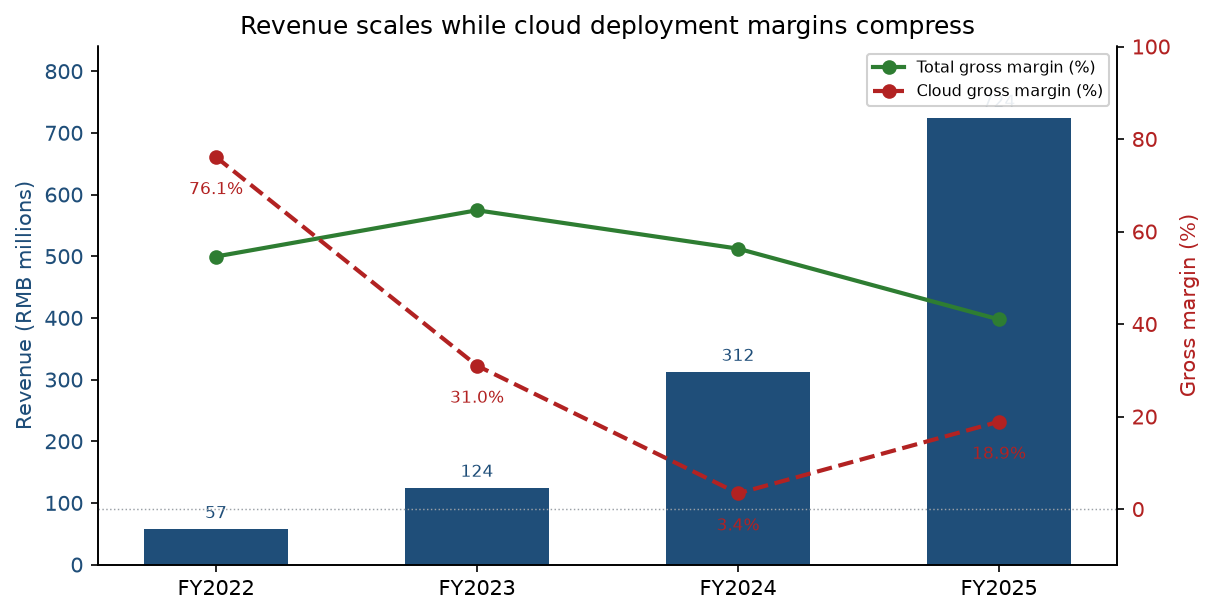
\includegraphics[width=0.82\textwidth]{fig8_financial_profile.png}
\caption{Zhipu's financial profile. H1 2026 is a six-month period and is not directly comparable with the
full-year bars. API gross margin recovered to 24.6\%, while the shift toward API revenue diluted total gross
margin to 26.4\%. Sources: Chapter~18C prospectus, 2025 annual report and 2026 interim results
\citep{prospectus2513,annualreport2513,interim2026}.}
\label{fig:fin}
\end{figure}

\textbf{Listing and market reaction.} Zhipu priced at HK\$116.20, raising about HK\$5.0bn after the
over-allotment option with HK\$3bn of cornerstone commitments, at an implied valuation near US\$6.7--7.4bn
\citep{prospectus2513,annualreport2513}. The listing is
strategically remarkable
on three counts: Chapter~18C gave a loss-making lab permanent public capital years before profitability; its
first-listed-foundation-model status conferred a certification premium; and the stock
then experienced a substantial re-rating followed by a reversal to HK\$780 by 18~September~2026 ($\approx +571\%$ versus IPO; realised annualised volatility
near 187\%; Figure~\ref{fig:price}). The company placed 19.78m new shares on 13~July at HK\$1{,}588,
raising HK\$31.375bn net and increasing issued shares from 445.843m to 465.623m
\citep{placement2513}. MiniMax, listing one day later at HK\$165, closed 18~September at HK\$303 after a much
larger peak-to-trough drawdown. Between 31~August and 11~September MiniMax fell 22.6\%, compared with
Zhipu's 33.6\%. In the following week, Zhipu fell another 1.6\% while MiniMax recovered 12.2\%.
Both rebounded after Tuesday; Friday gains were 5.4\% and 18.9\%, respectively. Partial mean reversion
therefore coexists with sharp recoveries and increasing peer divergence (Section~\ref{sec:event}).

\section{Industry, Macro, and Strategy}
\label{sec:context}
\textbf{Structure and strategy.} In Porter terms the foundation-model layer is harsh: supplier power
(advanced compute) is high and politically rationed, buyer switching costs are low because open weights
commoditise the layer, and the substitutes are rival open-weight models. Zhipu's answer is leaderboard
dominance through \emph{cost disruption}: a mixture-of-experts GLM-5 line (GLM-4.6: $\approx$355B parameters,
32B active, 200K context) that topped coding benchmarks---GLM-5.1 ranked \#1 on SWE-Bench Pro at 58.4\%, and
GLM-5.2 (June~2026) shipped with MIT open weights and a one-million-token context, followed by GLM-5.3
on 14~August and GLM-5.3-Flash on 26~August---priced below closed
competitors, now paired with nascent pricing power (8--17\% API price rises with each GLM-5.x release)
\citep{glm_modelcard,glm53,glm53flash}. Branch releases such as GLM-5V-Turbo are catalogued but excluded when they overlap
a main GLM window \citep{glm5v}. This cadence
defines the event taxonomy of Section~\ref{sec:event} (Figure~\ref{fig:timeline}). The main weakness is
self-inflicted: the same cadence commoditises its own product, while cloud-margin pressure and compute
dependence cap monetisation.

\begin{figure}[H]
\centering
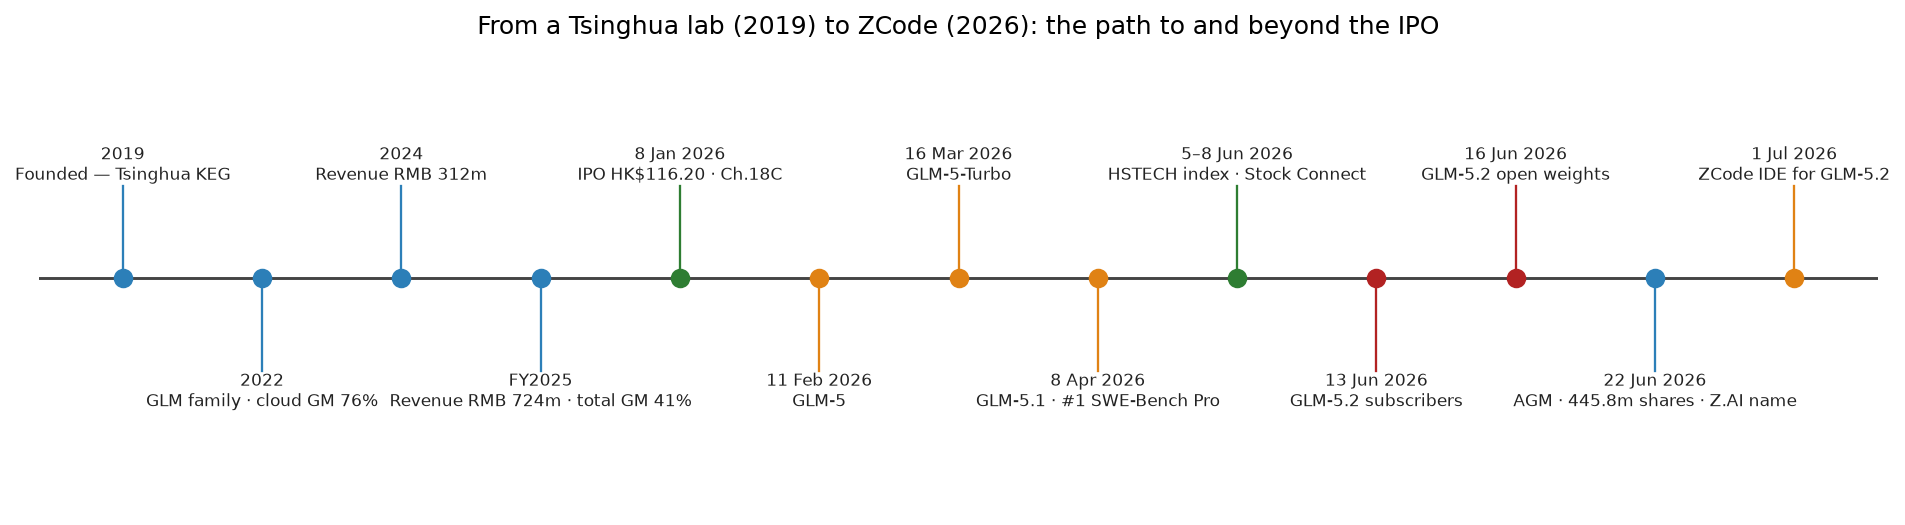
\includegraphics[width=\textwidth]{fig9_glm_timeline.png}
\caption{Company timeline from the 2019 founding through the 2026
Chapter~18C listing, July placement, GLM-5.3-Flash rollout and H1 results. Each open-weight launch is the unit of
\emph{capability surprise} studied in Section~\ref{sec:event} and the primary currency of value for an
early-commercial-stage lab; milestones are evenly spaced for legibility. Sources: Chapter~18C prospectus
\citep{prospectus2513}, official model documentation \citep{glm_modelcard}, placement announcement
\citep{placement2513}, and interim results \citep{interim2026}.}
\label{fig:timeline}
\end{figure}

\textbf{The Hong Kong AI-IPO landscape.} SenseTime (0020.HK), Fourth Paradigm (6682.HK), and Wenge AI
(01956.HK) give local AI context, but their vision, enterprise-ML, and decision-intelligence models differ from
a frontier laboratory \citep{prospectus20,prospectus6682,prospectus1956}. Moonshot AI (Kimi) and other Chinese
labs may eventually broaden the listed set. For now, \emph{MiniMax is the only direct listed comparable}
(Section~\ref{sec:rel}).

\textbf{Trust and distribution.} Model quality alone does not secure developer adoption. On 18~September,
developer ferstar alleged that ZCode uploaded workspace snapshots including Git history, with settings
that did not disable the upload path \citep{zcodeanalysis2026}. This paper has not independently reproduced
that analysis. In an evening response reported by IT Home, ZCode apologised, attributed uploads to the
default-enabled indexing/Repo Wiki feature, said the issue was fixed and data destroyed after Wiki
generation, and promised source release and external review \citep{zcoderesponse2026}. Those are company
claims, not independently verified deletion or audit results. The available evidence does not establish
that all repositories were successfully uploaded or used for training.

MiniMax Code CLI v0.4.12 was meanwhile released under MIT: a terminal coding-agent implementation that
can be inspected and extended, distinct from the older general-purpose MiniMax CLI and from model weights
\citep{minimaxcode2026}. Public source can reduce evaluation friction and improve distribution, but is not
itself a security certification or proof of incremental revenue.

The two developments belong to the same commercial contest for the developer workflow. ZCode's response
seeks to restore confidence in data handling; MiniMax's source release offers inspectability as a feature
of a competing coding tool. Read together, the controversy makes control over proprietary code more
salient, while an inspectable alternative may reduce the cost of evaluating another supplier. This is a
competitive interpretation, not evidence that MiniMax timed its release in response to ZCode. ZCode's
promise to open source and MiniMax's published tool source also differ in delivery status, although
neither alone verifies deployed behaviour.

The valuation link runs from data-control confidence through enterprise approval, developer trial and
switching decisions to retention and paid usage. Zhipu could face longer procurement cycles or remediation
costs; MiniMax could gain consideration without yet gaining revenue. Because the CLI supports other
models, tool adoption need not become MiniMax API consumption. These related commercial behaviours
therefore test whether capability-led repricing can become durable cash flow; no disclosed migration,
retention or loss estimate yet warrants a numerical DCF adjustment.

\textbf{Macro and flows.} Chinese AI is a policy priority (state/SOE demand); U.S. compute-export controls
force the architectural efficiency that doubles as Zhipu's cost edge; and Hong Kong's market structure sets
the marginal buyer. Zhipu joined the Hang Seng Tech Index on 5~June and Southbound Stock Connect on
8~June~2026, drawing about HK\$920m of net southbound buying on its first eligible day \citep{hsi2026}.
MSCI then added the H shares to its Emerging Markets and China indexes at the 31~August close
\citep{msci2026}. These flow events matter for Section~\ref{sec:event}, where we keep them separate from
capability and financial-disclosure events.

\section{Valuation}
\label{sec:val}

\subsection{Cost of capital}
We estimate the cost of equity with the CAPM. Zhipu's short post-IPO history makes its own regression beta
unstable, so we estimate 60-month monthly betas for global AI-software comparables against SPY through
31~August, unlever them, and round the 1.55 median to $\beta=1.6$ \citep{nasdaqsec2026}. With a risk-free
rate of 4.0\% and an equity risk premium of 6.0\%, $K_e = 4.0\% + 1.6\times 6.0\% = 13.6\%$; we retain a 13.5\% discount-rate benchmark for comparability. The new convertible debt does not justify
a mechanically cheaper rate: zero coupon is not zero economic financing cost. Throughout we use HK\$7.8/US\$, RMB~7.1/US\$, and
487.588m shares after the 16~September placement. The equity bridge adds \textbf{US\$6.308bn of
pro-forma net cash and short-term investments}: June cash and investments less bank loans and leases,
plus July and September placement net proceeds and September bond net proceeds, less an issue-date
bond-principal proxy \citep{interim2026,placement2513,zhipucompletion2026}. It is not a reported September
cash balance: subsequent operating burn is not disclosed. Appendix~\ref{sec:beta} records the beta bridge.

\textbf{Two caveats remain.} First, the beta set consists of mature software firms, while Zhipu resembles a
pre-profit, capital-intensive lab; the resulting WACC is generous. Second, fixing WACC at 13.5\% through 2035
ignores the risk-premium increase that could follow a break in the valuation loop. Both refinements would lower
DCF value. Figure~\ref{fig:tornado} tests rate sensitivity, while the real-options section treats the binary tail.

\textbf{Financing and valuation treatment.} The 18~September completion announcement confirms that
21,965,000 new H shares at HK\$714 were placed on 16~September, raising HK\$15,664.13m net; RMB20.14bn
of US-dollar-settled zero-coupon convertible bonds were issued on 18~September, raising US\$3,010.77m
net \citep{zhipucompletion2026}. The earlier 9.96\% placement discount refers to the 11~September HK\$793
close. Initial conversion is at HK\$892.50; maturity is 16~September~2027, with the ordinary conversion
period beginning on 1~July~2027 \citep{zhipufinancing2026}.

The bridge now recognises completion, replacing the previous conditional treatment. It adds net proceeds
but deducts US\$3,000.64m for the bond claim, calculated as disclosed US\$3,015.64m gross proceeds divided
by the 100.5\% issue price. This is an issue-date principal proxy, not an IFRS fair-value estimate;
actual dollar settlement depends on the bond terms and exchange rates. No option value is separately
estimated. A non-conversion treatment uses 487.588m shares; full conversion at the initial price would
increase shares to 513.953m and remove the corresponding debt claim. The model does not combine both
full dilution and a debt deduction. Completed financing increases the weighted DCF from roughly HK\$88
to HK\$116 with operating assumptions unchanged; it does not demonstrate better operating profitability.
Zero coupon also leaves a near-term repayment or refinancing obligation. The proposed use of 60\% of
net proceeds for GLM development and infrastructure links funding capacity to future execution risk.

\subsection{Scenario DCF}
We project FCFF over 2026--2035 from a \textbf{US\$700m FY2026E revenue base}. That figure is our estimate,
not company guidance. It starts from reported H1 revenue of RMB~953.9m and implies RMB~4.02bn in H2; the
step-up is demanding, though below the August run-rate reported by management after the results
\citep{interim2026,caixin2026}. Revenue growth then fades from a scenario-specific 2027 rate to maturity.
Operating margin begins at $-100\%$---still a sharp improvement from H1's $-225\%$---and converges toward a
terminal level. The model applies a 15\% tax rate, reinvestment through a sales-to-capital ratio of 1.6--2.0,
and terminal growth of 4\%. When EBIT is negative, cash tax is zero and losses build a simple NOL
carryforward; positive EBIT is taxed only after that balance is absorbed. Appendix~\ref{sec:proj} reports the
full Base-case chain, and Table~\ref{tab:dcf} gives the headline results.

\begin{table}[H]
\centering
\caption{Three-scenario DCF (USD unless noted; per-share in HKD). Market row at the 18~September close. Operating assumptions are unchanged.}
\label{tab:dcf}
\begin{tabular}{lcccc}
\toprule
Scenario & Rev.\ CAGR '26--35 & Term.\ margin & Equity value & Per share (HK\$) \\
\midrule
Bear ($p=0.35$) & 23\% & 18\% & US\$3.5B & 56 \\
Base ($p=0.45$) & 31\% & 28\% & US\$6.4B & 102 \\
Bull ($p=0.20$) & 47\% & 35\% & US\$15.9B & 255 \\
\midrule
\textbf{Probability-weighted} & --- & --- & \textbf{US\$7.3B} & \textbf{116} \\
\midrule
\textit{Market (2026-09-18)} & --- & --- & \textit{US\$48.8B} & \textit{780} \\
\bottomrule
\end{tabular}
\end{table}

The probability-weighted intrinsic value is HK\$116 per share---roughly \textbf{14.9\% of the market price}.
The H1 evidence lifts the valuation starting point, but the quoted price still requires a much larger outcome
than this conventional cash-flow model.

\subsection{Reverse DCF: what the price requires}
We invert the model to ask what justifies the US\$48.8bn equity value while holding FY2026E revenue fixed.
At WACC~13.5\% and a 40\% terminal margin, the price requires \textbf{about US\$59.7bn of 2035 revenue}:
2027 growth of roughly 130\%, followed by a path that still compounds at 63.9\% from 2026 to 2035.
Figure~\ref{fig:revheat} grids WACC (10--20\%) against terminal margin (20--50\%). Even the most favourable
cell (10\%/50\%) requires about US\$19bn, while 15\%/40\% requires US\$84bn. The reverse DCF is therefore
less a target price than a statement of the right-tail outcome already embedded in the quote.

\begin{figure}[H]
\centering
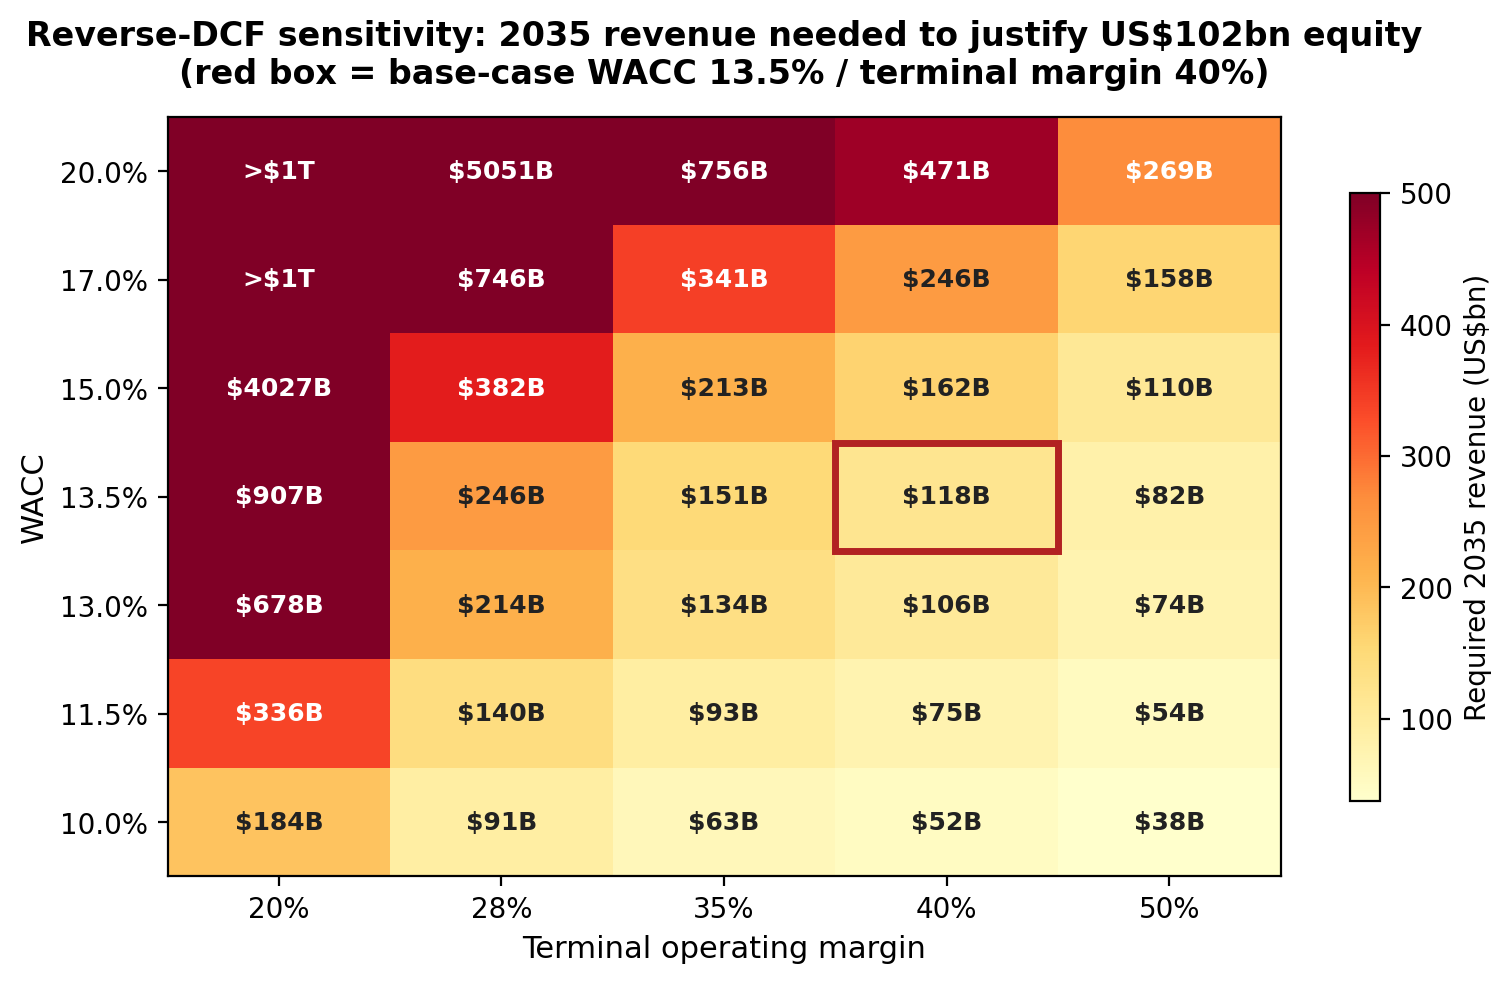
\includegraphics[width=0.82\textwidth]{fig11_reverse_dcf_heatmap.png}
\caption{Reverse-DCF sensitivity: 2035 revenue (US\$bn) required to justify the US\$48.8bn equity value
across WACC and terminal-margin assumptions. The red box marks the base case (13.5\%/40\%). Data:
Table~\ref{tab:revheat} in Appendix~\ref{sec:revheat}.}
\label{fig:revheat}
\end{figure}

\subsection{Relative valuation}
\label{sec:rel}
We divide each listed lab's 18~September equity value by LTM revenue through 2026H1. Zhipu's RMB~1{,}487.3m
(FY2025 less H1~2025 plus H1~2026), or US\$209.5m at RMB7.1/US\$, gives \textbf{232.8$\times$}.
MiniMax's US\$13.57bn equity value and US\$165.2m LTM revenue give \textbf{82.1$\times$}. Private transactions imply
\textbf{34.1$\times$} for OpenAI, \textbf{20.5$\times$} for Anthropic, and \textbf{39.0$\times$} for Mistral
\citep{minimax2026h1,openai2026,anthropic2026,mistral2025}. This private range, with a 34.1$\times$ median, is
the football-field transaction range. Their revenue run-rates apply separately to Zhipu's FY2026E estimate,
giving HK\$230--437 per share. MiniMax's LTM multiple applied to Zhipu's LTM revenue gives HK\$275.

MiniMax's 26~August results anchor the peer denominator. H1 revenue rose 283.1\% to US\$116.6m and gross margin
reached 17.9\%, while adjusted net loss doubled to US\$293.0m. Its US\$165.2m LTM revenue equals FY2025 less
H1~2025 plus H1~2026, rather than annualised H1 revenue \citep{minimax2026h1}.

SenseTime, Phancy, and Wenge are Hong Kong adjacent-AI references; Palantir, Cloudflare, and Snowflake represent
commercialisation \citep{hkcomps2026,softwarecomps2026}. Different economics make both groups context only.
On the matched basis, Zhipu's multiple is 2.83 times MiniMax's, so the peer supports far less of the quote
(Figure~\ref{fig:comps}).

\begin{figure}[H]
\centering
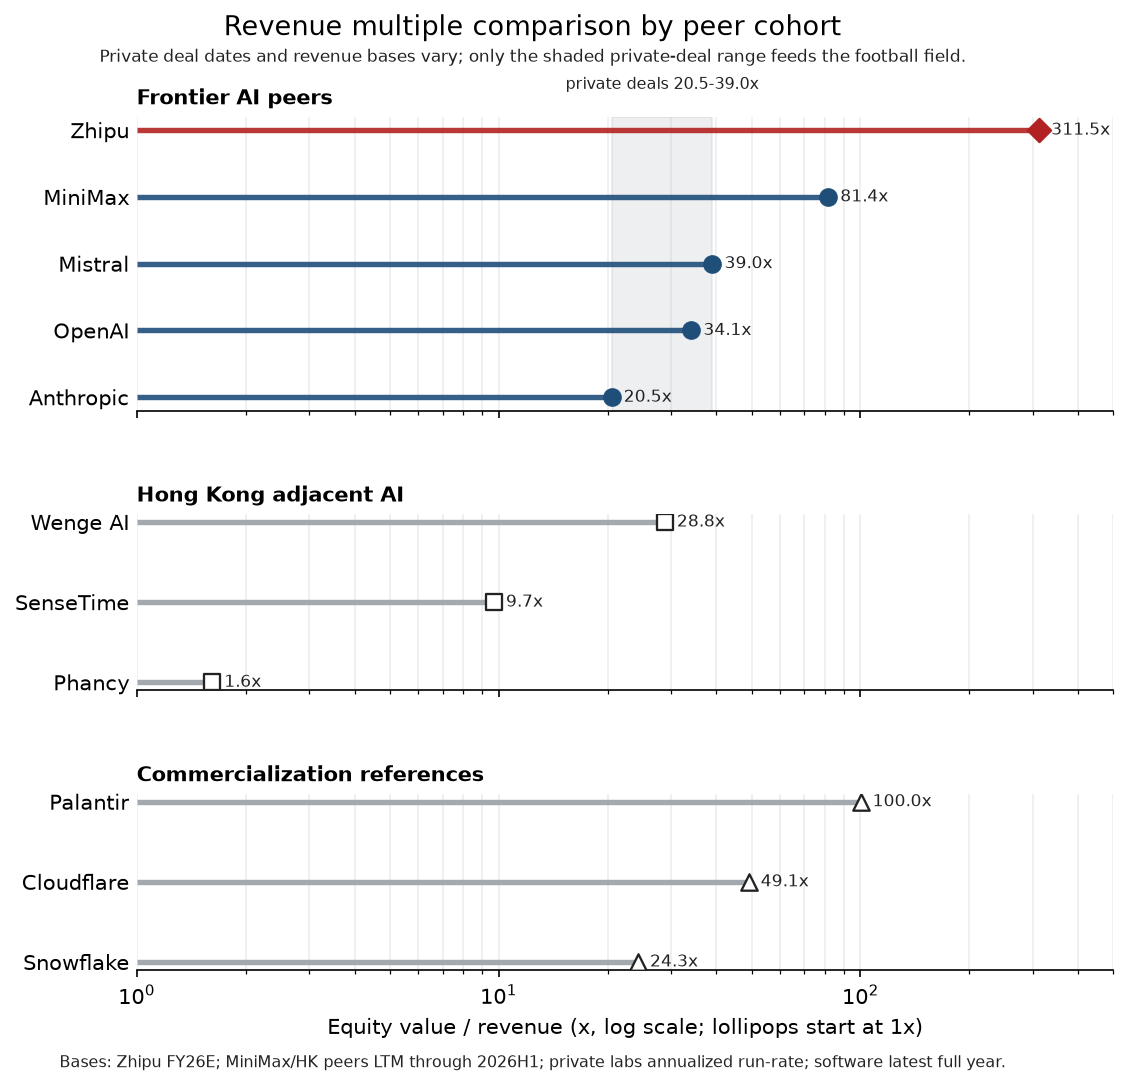
\includegraphics[width=0.96\textwidth]{fig6_ps_comps.png}
\caption{Layered equity value / revenue multiples (log scale). The chart shows core frontier peers, Hong
Kong adjacent-AI firms, and commercialisation references in separate groups. Only the shaded private-deal
range from 20.5$\times$ to 39.0$\times$ feeds the football field. Zhipu, MiniMax, and the Hong Kong listed peers
use LTM revenue through 2026H1; each other revenue period is recorded in \texttt{data/valuation\_comps.csv}.}
\label{fig:comps}
\end{figure}

\textbf{Wenge's interim cross-check.} Wenge's 25~August interim-results announcement reports H1 revenue
of RMB172.750m, up 46.0\%; deployment contributes RMB113.803m (65.9\%), while subscription and API revenue
reaches RMB58.947m (34.1\%), up 94.0\% \citep{wengeh12026}. Gross margin is 55.0\%, versus 54.6\% a year
earlier. R\&D expense rises 59.0\% to RMB119.340m, or 69.1\% of revenue. Its deployment-heavy delivery
model and margin profile differ substantially from Zhipu's API-heavy mix; Wenge therefore remains an
adjacent Hong Kong comparable, outside the private foundation-lab valuation range.

Loss measures must be distinguished. Total period loss narrows 24.5\% to RMB87.654m; loss attributable
to owners narrows 27.6\% to RMB88.958m; adjusted net loss narrows 29.5\% to RMB52.920m. Financial-asset
fair-value gains increase from RMB0.200m to RMB35.047m, contributing to reported loss improvement.
Cash and cash equivalents increase from RMB324.621m at year-end to RMB1,017.608m in June; the broader
liquidity increase is primarily attributable to IPO proceeds, rather than evidence of positive operating
cash flow. Growth and adjusted-loss improvement are encouraging, but R\&D still grows faster than revenue.
The comparable table already uses an H1-updated LTM denominator; these disclosures are not added a second
time. The source is the formal interim-results announcement, not a separately verified full interim report.

\subsection{A real-options reading}
The valuation gap can be interpreted as investors paying for a \emph{call option
on a winner-take-all AGI outcome} \citep{black1973,damodaran2018}. This is an economic analogy, not an independently estimated option price: the gap above DCF reflects
expectations about a fat right tail. Roughly 187\% annualised volatility also means that this expectations
premium can contract sharply without technical progress being reversed. The reverse DCF describes the state needed for that option to pay off, while
Section~\ref{sec:event} tests how capability news changes its perceived probability.

\textbf{A practitioner lens: reflexivity.} This also fits Feng Liu's reverse-investing interpretation of
Soros's \emph{reflexivity} \citep{fengliu}. A high valuation is an input as well as an output: cheap equity
capital finances compute and talent, which can improve models and support the valuation. The July placement
makes that loop tangible. It remains fragile because the firm does not yet fund itself; if capability surprises
or monetisation stall, the same loop can reverse. September's HK\$714 placement price, against July's
HK\$1,588, illustrates how the terms of equity finance change as the market reprices. The transactions
have different dates and terms, so this comparison is descriptive. Continued access to capital supports
research, while dilution and debt repayment constrain how much of future success accrues to each share.

\subsection{Sensitivity and synthesis}
The conclusion is not an artefact of any single assumption. Figure~\ref{fig:tornado} tornadoes the Base case
against its main drivers. One-at-a-time changes put the Base case between roughly HK\$74 and HK\$131: useful
for locating model risk, but insufficient to bridge the gap to market. Figure~\ref{fig:ff} draws the whole
picture together. Scenario DCF spans HK\$56--255, the 20.5--39.0$\times$ private-deal range gives HK\$230--437,
and MiniMax's 82.1$\times$ LTM multiple gives about HK\$275 when applied to Zhipu's LTM revenue. That anchor is
64.7\% below Zhipu's HK\$780 close. Public markets value both listed labs richly, but Zhipu still carries a
2.83-fold multiple premium to MiniMax. Thus the observed decline is a partial compression of the
expectations premium, not evidence that the price has already returned to fundamental value. Neither
HK\$116 nor a historical average is an empirically established long-run mean.

\begin{figure}[H]
\centering
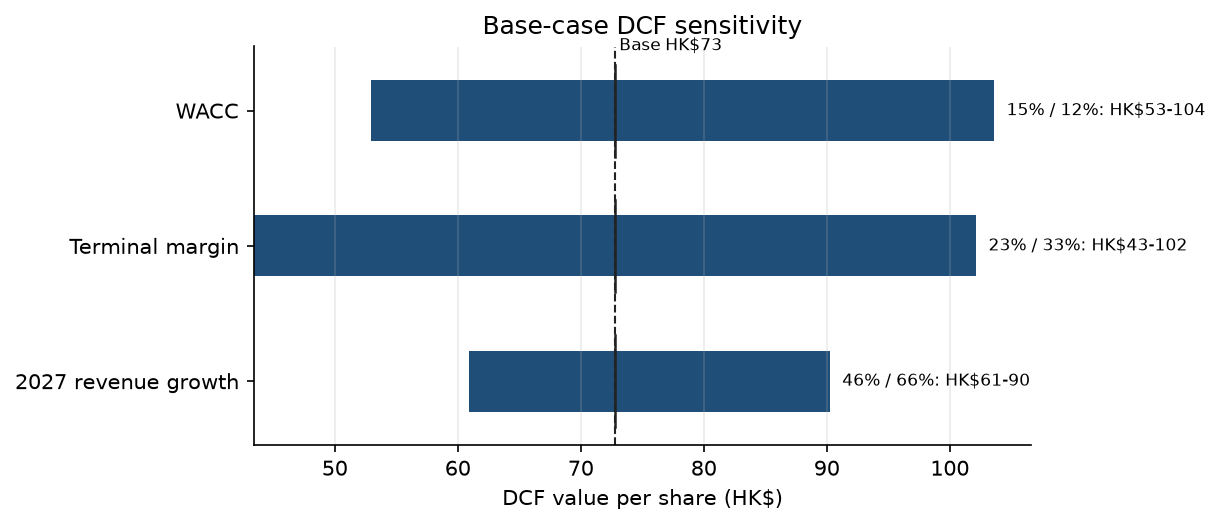
\includegraphics[width=0.82\textwidth]{fig7_sensitivity.png}
\caption{DCF sensitivity (Base case, per share). Bars span each driver's low/high setting around the
HK\$102 base; no one-at-a-time input change moves value near the market price.}
\label{fig:tornado}
\end{figure}

\begin{figure}[H]
\centering
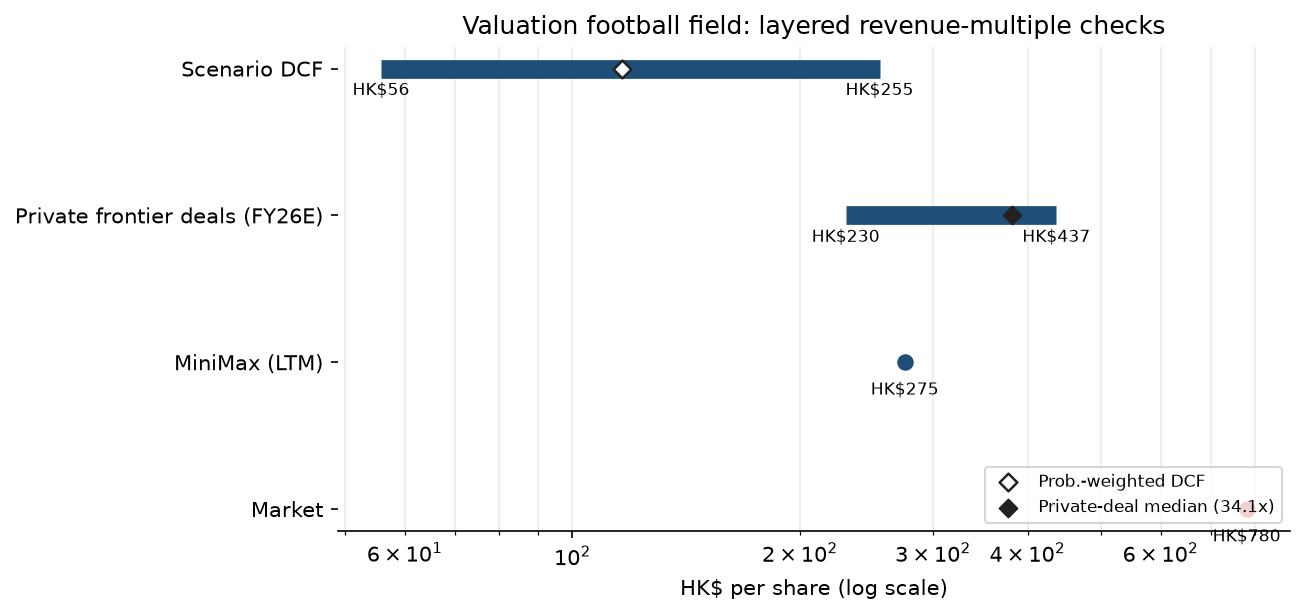
\includegraphics[width=0.86\textwidth]{fig5_football_field.png}
\caption{Valuation football field (log scale). The private-deal range and MiniMax's public LTM multiple are
shown separately; the diamonds mark probability-weighted DCF and the private-deal median.}
\label{fig:ff}
\end{figure}

\section{Capability Surprise: An Event Study}
\label{sec:event}
\textbf{Hypothesis.} If the firm is priced on its capability trajectory, then capability information should
move the price. Under semi-strong efficiency \citep{fama1970} the reaction should be immediate and complete;
subsequent continuation may reflect gradual adjustment, while reversal may reflect an initially excessive
response or adverse intervening information. We therefore examine both \emph{post-capability-announcement
drift} (PCAD), analogous to post-earnings-announcement drift\citep{ball1968,bernard1989}, and mean-reversion
patterns. Neither direction alone proves inefficiency when expected returns and other news are uncertain.

\textbf{Method.} Event dates are identified \emph{independently} from official model-release announcements and
technical documentation \citep{glm_modelcard,minimax_m3}, not from the price series. On daily prices
\citep{tushare2026,yfinance2026}
we compute mean-adjusted abnormal returns and CARs over three windows---leakage $[-5,-1]$, reaction $[0,+1]$,
and drift $[+2,+10]$---following standard event-study practice \citep{mackinlay1997} and the surprise-event
design of Guosen Securities\citep{guosen2020}. For each event the expected daily return is Zhipu's mean return over the
pre-event estimation window $[-20,-6]$, and the abnormal return is
$AR_t = R_t - \overline{R}_{[-20,-6]}$. Figure~\ref{fig:rets} then serves as a \emph{descriptive cross-check}:
several of the largest positive-return days coincide with these independently dated capability events.

\begin{figure}[H]
\centering
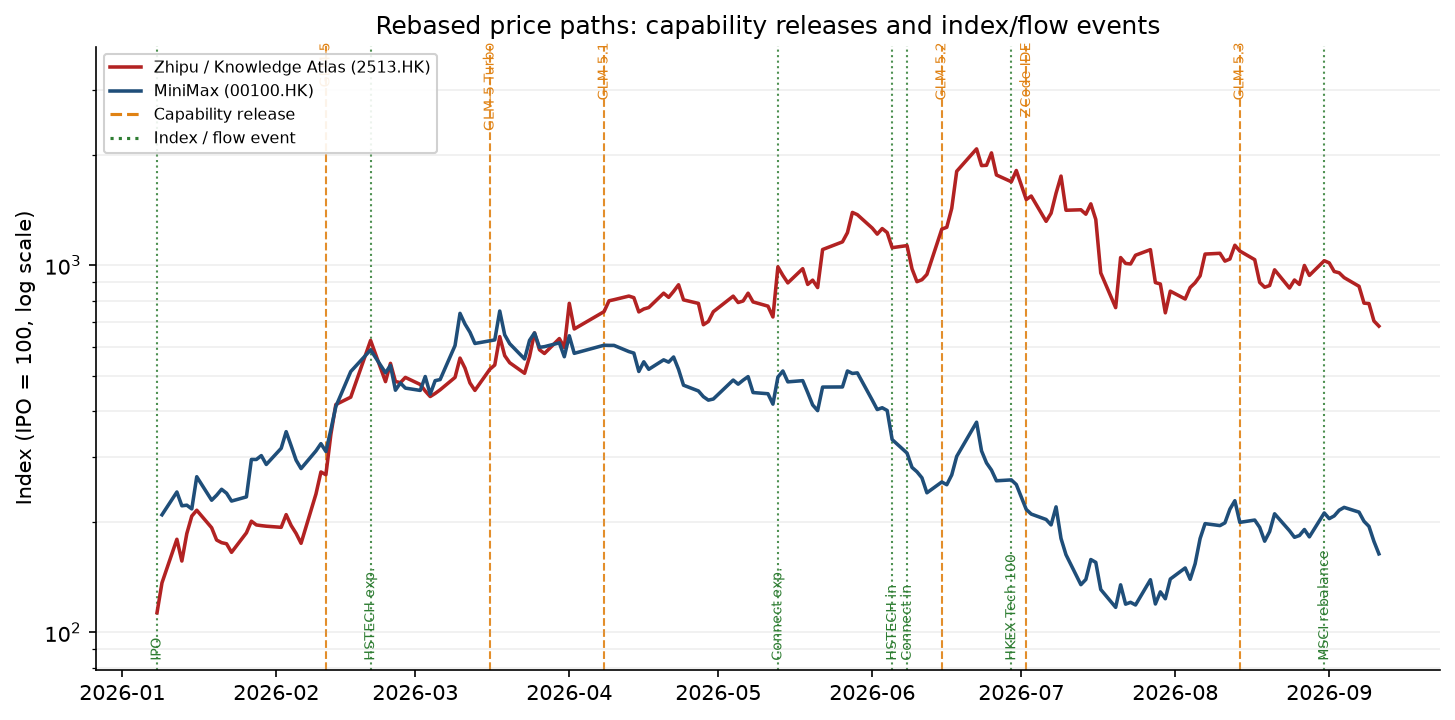
\includegraphics[width=0.88\textwidth]{fig1_price_paths.png}
\caption{Rebased prices (IPO~$=100$, log scale, through 2026-09-18). Orange dashed lines mark capability
releases (GLM-5 through GLM-5.3); green dotted lines mark index/flow catalysts (IPO, the 20~Feb and 13~May
expectation spikes, the 5--8~June Hang Seng TECH inclusion and Stock Connect access, and the 31~August MSCI
rebalance). Same sector,
divergent earlier paths, followed by a common September reversal: Zhipu loses part of its capability premium while MiniMax also declines.}
\label{fig:price}
\end{figure}

\begin{figure}[H]
\centering
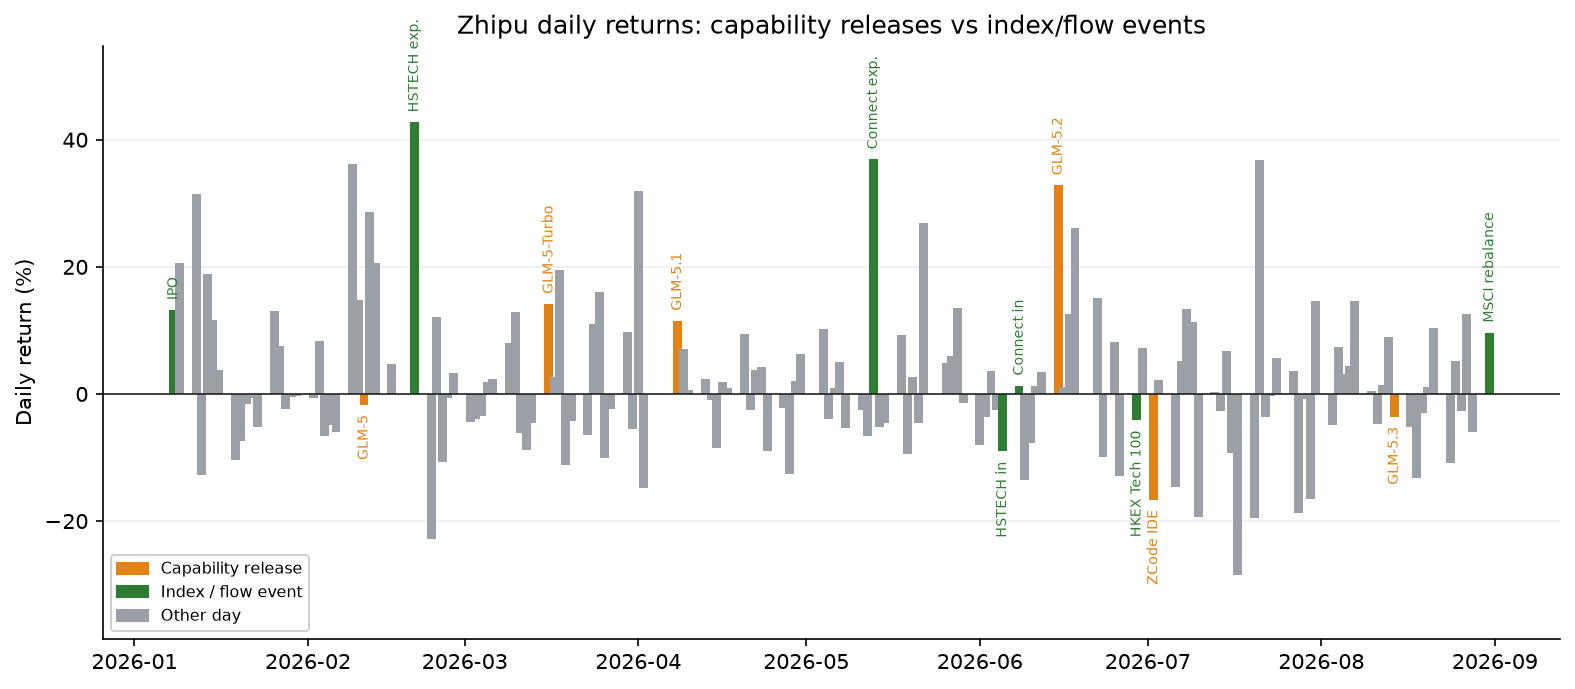
\includegraphics[width=0.88\textwidth]{fig2_daily_returns.png}
\caption{Descriptive cross-check: Zhipu's daily returns with capability-release days (orange) and index/flow
days (green) highlighted. Several of the largest up-days coincide with independently dated GLM releases, but the
two biggest---$+43\%$ on 20~Feb and $+37\%$ on 13~May---are index/flow events, not model releases. (Event
dates are taken from official announcements and index/Connect schedules, not from this chart.)}
\label{fig:rets}
\end{figure}

\textbf{Results.} Averaged across the five GLM events, the reaction window is $+13.7\%$ (the market prices
capability quickly) and the drift averages $+4.6\%$ but is strongly \emph{bimodal} (Table~\ref{tab:car}).
Within this small sample, the SOTA leap GLM-5.2 is followed by continuation, whereas
incremental upgrades (GLM-5-Turbo, GLM-5.1) reverse. MiniMax M2.5 drew a $+24.2\%$ launch reaction with little
subsequent drift, whereas M2.7 and M3 both drew negative reaction/drift profiles. That contrast is consistent with
\emph{heterogeneous responses to capability news}, without establishing a permanent return premium
(Figures~\ref{fig:car}--\ref{fig:scatter}).

\begin{table}[H]
\centering
\caption{Cumulative abnormal returns around capability events (mean-adjusted, \%; data through
31~August~2026).}
\label{tab:car}
\scriptsize
\setlength{\tabcolsep}{4pt}
\renewcommand{\arraystretch}{0.82}
\begin{tabular}{lcccc}
\toprule
Event & Day 0 & Reaction $[0,+1]$ & Drift $[+2,+10]$ & Reading \\
\midrule
GLM-5 & 2026-02-11 & $+22.5$ & $+24.7$ & under-reaction \\
GLM-5-Turbo & 2026-03-16 & $+7.7$ & $-19.3$ & reversal \\
GLM-5.1 & 2026-04-08 & $+13.8$ & $-14.2$ & over-reaction \\
GLM-5.2 & 2026-06-15 & $+30.8$ & $+28.2$ & strong under-reaction \\
GLM-5.3 & 2026-08-14 & $-6.5$ & $+3.8$ & anticipated / delayed reaction \\
\midrule
MiniMax M2.5 & 2026-02-12 & $+24.2$ & $-2.1$ & front-loaded reaction \\
MiniMax M2.7 & 2026-03-18 & $-5.5$ & $-49.1$ & de-rate \\
MiniMax M3 & 2026-06-01 & $-21.1$ & $-40.8$ & failed catalyst \\
\midrule
\multicolumn{5}{l}{\emph{Large-tech AI comparators}}\\
Baidu ERNIE 5.0 & 2026-02-06 & $-0.4$ & $-15.8$ & de-rate \\
Baidu ERNIE 5.1 & 2026-05-11 & $-5.0$ & $-13.6$ & de-rate \\
Alibaba Qwen3.5 & 2026-02-16 & $-4.5$ & $-10.9$ & de-rate \\
Alibaba Qwen3.6 & 2026-04-16 & $+6.5$ & $-5.5$ & reversal \\
Alibaba Qwen3.7-Max & 2026-05-21 & $-3.4$ & $-2.1$ & de-rate \\
Alibaba Qwen3.7-Plus & 2026-06-01 & $+8.6$ & $-15.9$ & reversal \\
Alibaba Qwen3.8-Max & 2026-08-03 & $+5.3$ & $-12.8$ & reversal \\
Tencent Hunyuan 3.0 preview & 2026-04-22 & $-4.2$ & $-1.3$ & de-rate \\
Tencent Hy3 & 2026-07-06 & $+8.2$ & $+9.8$ & under-reaction \\
Meituan LongCat-2.0 & 2026-06-30 & $+4.8$ & $+17.3$ & under-reaction \\
Google Gemini 3.1 Pro & 2026-02-19 & $+4.0$ & $-4.0$ & reversal \\
Google Gemini 3.5/Omni & 2026-05-19 & $-4.0$ & $-16.7$ & de-rate \\
Google Gemini 3.6 Flash & 2026-07-21 & $-2.3$ & $+13.0$ & delayed reaction \\
Google Gemini 3.7 Flash & 2026-08-13 & $+0.9$ & $-0.7$ & muted \\
Meta Muse Spark & 2026-04-08 & $+11.5$ & $+18.2$ & under-reaction \\
Meta Muse Spark 1.1 & 2026-07-09 & $+11.1$ & $-7.6$ & reversal \\
Microsoft/OpenAI GPT-5.5 proxy & 2026-04-23 & $-3.2$ & $-6.9$ & de-rate \\
Microsoft/OpenAI GPT-5.6 proxy & 2026-07-09 & $+1.7$ & $+4.9$ & muted continuation \\
Microsoft/OpenAI GPT-5.6 Aug. proxy & 2026-08-06 & $+2.3$ & $-5.0$ & reversal \\
Tesla/xAI Grok 4.3 Beta proxy & 2026-04-17 & $+2.6$ & $+7.0$ & muted continuation \\
Tesla/xAI Grok 4.5 proxy & 2026-07-20 & $-1.0$ & $-17.3$ & de-rate \\
Tesla/xAI Grok 4.6 proxy & 2026-08-12 & $+4.6$ & $+12.6$ & under-reaction \\
\midrule
\textbf{Average (22 large-tech)} & & $\mathbf{+2.0}$ & $\mathbf{-2.4}$ & \\

\textbf{Average (5 GLM)} & & $\mathbf{+13.7}$ & $\mathbf{+4.6}$ & \\
\bottomrule
\end{tabular}

{\footnotesize Mean-adjusted abnormal return: $AR_t=R_t-\bar{R}_{[-20,-6]}$, where
$\bar{R}_{[-20,-6]}$ is the average raw return over event days $-20$ through $-6$. Comparator dates are pinned
to primary-source release announcements or model cards
\citep{minimax_m25,minimax_m3,minimax_media,ernie50,ernie51,qwen35,qwen36,qwen38,tencenthy,meituanlongcat,geminiio2026,geminiflash,metamuse,musespark11,gpt55,gpt56,grokchatbot,grokofficial}.
Weekend announcements use the next trading day. OpenAI and xAI releases remain in the audit catalogue, but
Microsoft and Tesla returns are excluded because neither listed company is the model issuer. Same-week Qwen3.8
variants are catalogued but not double-counted after the 3~August flagship launch. Qwen3.8-Flash (26~August), Gemini
Transcribe/Omni 1.1 (26--27~August), Tencent Hy4 (28~August), GLM-5.3-Flash, the two H1 disclosures, and MSCI
rebalance lacked a complete post-event window at the original 31~August sample cutoff and remain outside this historical table. Later observable windows are analysed below. MiniMax H3 and Music
3.0 remain catalogued but are excluded because audio-video and music generation are not comparable with the
text, coding, and agent capability sample.}
\renewcommand{\arraystretch}{1.0}
\setlength{\tabcolsep}{6pt}
\end{table}

\begin{figure}[H]
\centering
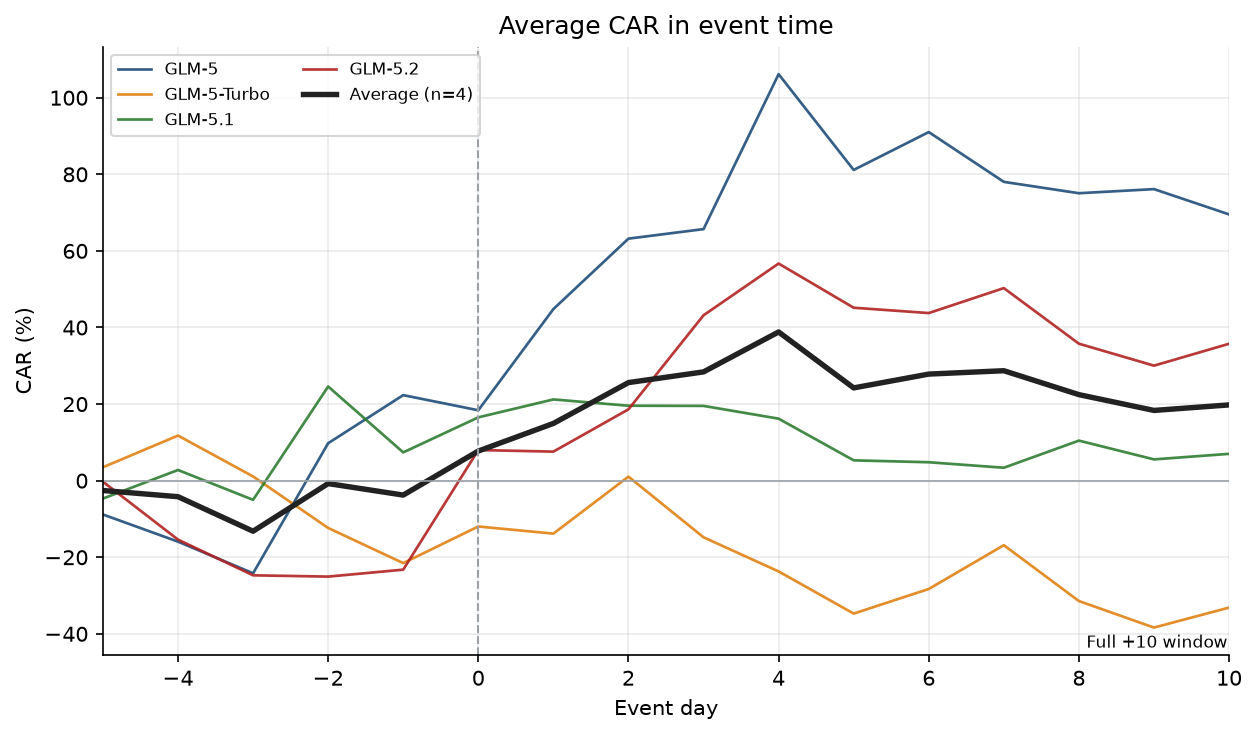
\includegraphics[width=0.72\textwidth]{fig3_car_eventtime.png}
\caption{Average CAR in event time across the five GLM events (mean-adjusted, $[-20,-6]$ estimation window).
The average is plotted where all five GLM events have data through the full $[+2,+10]$ drift window.}
\label{fig:car}
\end{figure}

\begin{figure}[H]
\centering
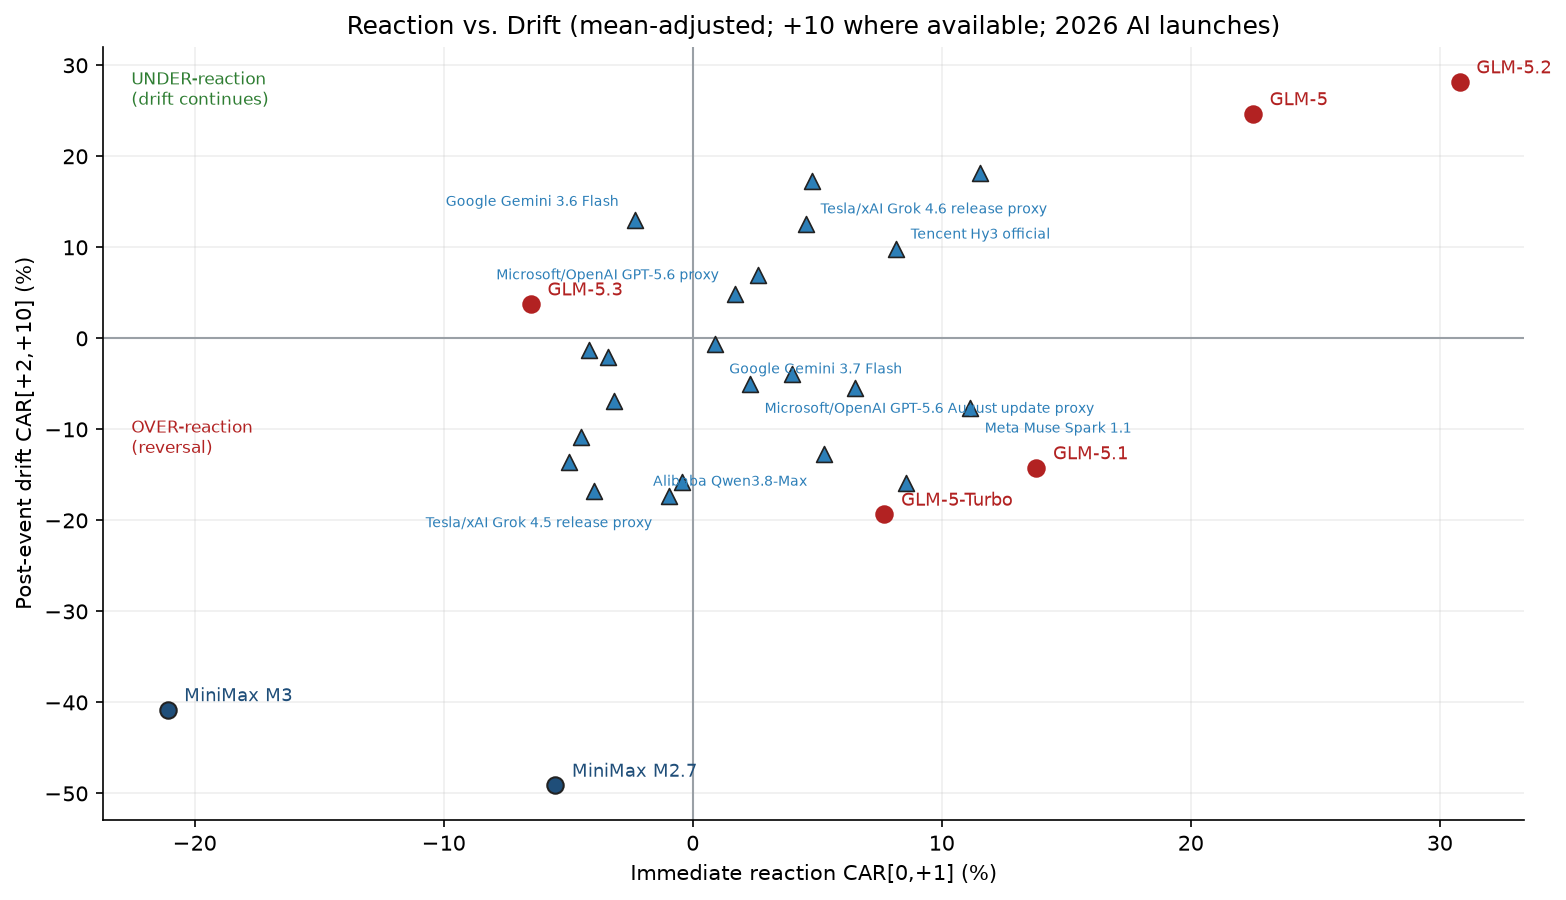
\includegraphics[width=0.86\textwidth]{fig4_reaction_vs_drift.png}
\caption{Reaction versus drift. SOTA leaps sit in the under-reaction quadrant; incremental upgrades in the
over-reaction quadrant. Triangle markers show large-tech AI comparators.}
\label{fig:scatter}
\end{figure}

\subsection{Not every spike is capability: flow events}
Two of the largest blind-detected up-days do \emph{not} map to a model release: $+43\%$ on 2026-02-20 and
$+37\%$ on 2026-05-13. Both coincide with \emph{index/flow} catalysts---rising expectations of Hang Seng Tech
inclusion and Stock Connect access (realised 5~and 8~June). Separating capability events from flow events
matters: the CARs above are driven by the former, while the latter explain part of the raw volatility and warn
against attributing every move to model quality. The same discipline matters at the new cutoff. Zhipu rose
9.6\% on 31~August as MSCI's index changes became effective after the close \citep{msci2026}; the H1 results
were released only after that close \citep{interim2026}. The financial disclosure can update valuation inputs,
but it cannot explain that day's return. By 18~September its supplementary drift window is complete (nine days, -54.4\% mean-adjusted CAR),
but it remains a financial event outside the original capability sample. That CAR overlaps other news
and is not an isolated estimate of the results' effect. The 13~September financing announcement
likewise follows the measured drawdown; it cannot retrospectively establish its cause.

\subsection{Robustness: peer-adjusted and block-bootstrap checks}
Because Zhipu and MiniMax share sector and macro shocks, we re-run the study with \emph{peer-adjusted} returns
(benchmark $=$ MiniMax's same-day return). Table~\ref{tab:robust} shows the reaction result is highly robust
($+13.7\%$ vs $+15.3\%$), while the average drift \emph{strengthens} ($+4.6\%\!\to\!+16.8\%$): once the falling
sector is removed, all five events drift positively, and GLM-5.1's apparent reversal flips to continuation
($-14.2\%\!\to\!+12.9\%$). This shows relative strength against a falling peer in the original windows. It does not imply that
absolute prices will keep rising, and the bootstrap below does not establish significant continuation.

An expanded event catalogue guards against cherry-picking by recording screened releases, financial disclosures,
flow catalysts, listings, and candidates. Twenty-nine day-level, clean-window events enter the CAR panel;
exclusions carry explicit reasons. Capability reactions remain positive, while flow events show weaker reactions
but stronger drift, supporting their separate treatment.

\begin{table}[H]
\centering
\caption{Robustness: mean-adjusted vs peer-adjusted CAR (\%).}
\label{tab:robust}
\begin{tabular}{lcccc}
\toprule
 & \multicolumn{2}{c}{Mean-adjusted} & \multicolumn{2}{c}{Peer-adjusted} \\
\cmidrule(lr){2-3}\cmidrule(lr){4-5}
Event & React $[0,1]$ & Drift $[2,10]$ & React $[0,1]$ & Drift $[2,10]$ \\
\midrule
GLM-5 & $+22.5$ & $+24.7$ & $+17.2$ & $+13.3$ \\
GLM-5-Turbo & $+7.7$ & $-19.3$ & $+14.6$ & $+19.2$ \\
GLM-5.1 & $+13.8$ & $-14.2$ & $+13.4$ & $+12.9$ \\
GLM-5.2 & $+30.8$ & $+28.2$ & $+28.7$ & $+36.8$ \\
GLM-5.3 & $-6.5$ & $+3.8$ & $+2.4$ & $+1.8$ \\
\midrule
\textbf{Average} & $+13.7$ & $+4.6$ & $+15.3$ & $+16.8$ \\
\bottomrule
\end{tabular}

{\footnotesize Mean-adjusted uses Zhipu's pre-event average return over $[-20,-6]$; peer-adjusted uses
MiniMax's same-day return as the benchmark. All five GLM drift windows are complete through $+10$.}
\end{table}

\textbf{Block-bootstrap check.} With only five events, a parametric $t$-test would create false precision. We
therefore draw 20{,}000 non-event peer-adjusted return blocks with numpy.random.choice, preserving the
two-day reaction and nine-day drift window lengths, and compare the actual five-event mean CAR with the
bootstrap mean distribution (Figure~\ref{fig:boot}). The actual peer-adjusted reaction ($+15.3\%$) sits above
the 95\% null interval ($[-14.0,+12.6]\%$) and at the 99.2nd percentile. Drift ($+16.8\%$) is positive but
inside its wider null interval ($[-22.8,+25.5]\%$), at percentile 88.0. Thus the block bootstrap supports
a strong immediate capability reaction and only directional, not statistically conclusive, continuation.

\begin{figure}[H]
\centering
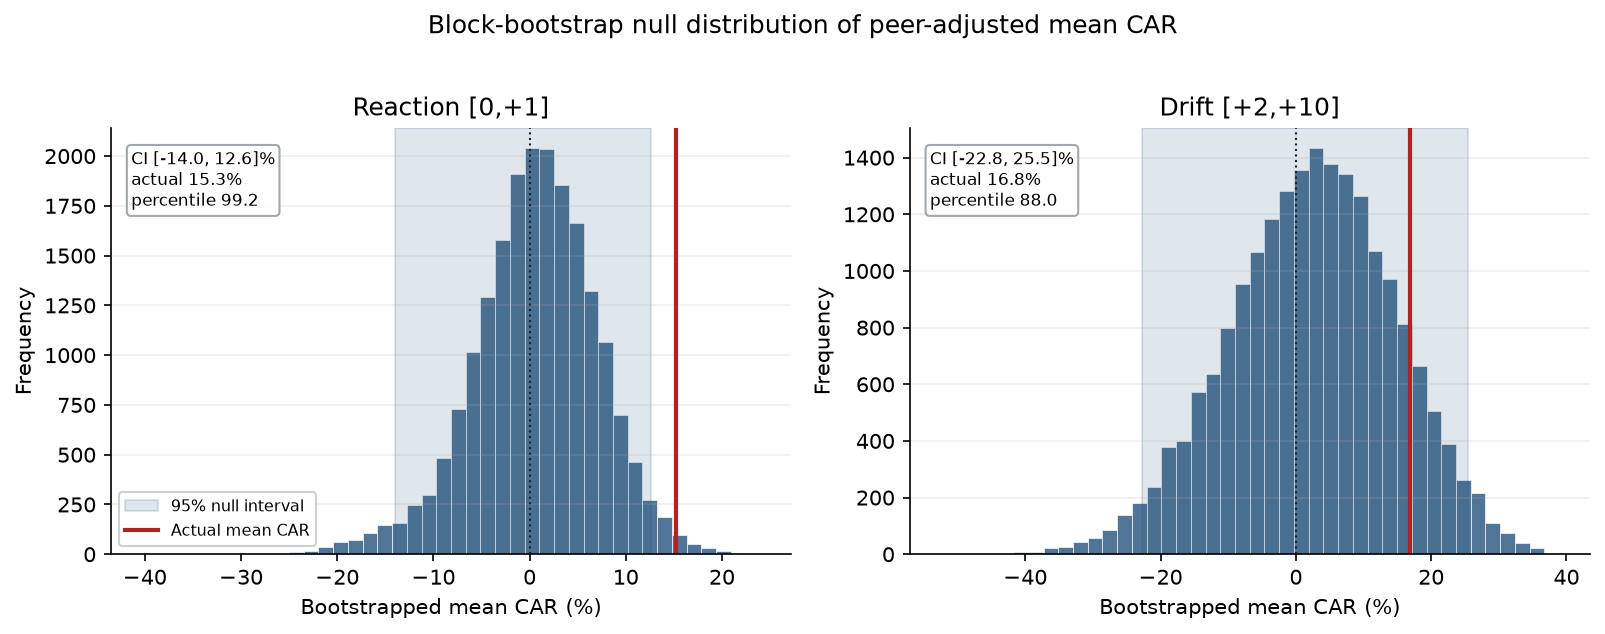
\includegraphics[width=0.92\textwidth]{fig10_block_bootstrap.png}
\caption{Block-bootstrap null distributions for peer-adjusted mean CAR. Each draw samples five non-event
return blocks with replacement using numpy.random.choice; block lengths match the actual event
windows. Shaded areas are percentile 95\% null intervals, and red lines mark the actual five-event means.}
\label{fig:boot}
\end{figure}

\subsection{From capability revaluation to partial mean reversion}
The September observations change the interpretation of the earlier positive reactions. GLM-5.3-Flash
has a +9.1\% two-day mean-adjusted reaction but -25.9\% subsequent nine-day drift. MiniMax's interim-results
window similarly records -5.7\% reaction and -23.2\% drift. These complete supplementary windows, reported
in \texttt{eventstudy/september\_window\_update.csv}, show that capability or commercialisation news need
not sustain its initial valuation effect. They are separate from the fixed August five-event estimates.

Over 31~August--11~September, Zhipu's raw decline of 33.6\% exceeds MiniMax's 22.6\% decline by roughly
11 percentage points. These calendar-period returns are distinct from event CARs. Together they are
consistent with a common repricing and an additional compression of Zhipu's premium; a single-peer
comparison cannot identify the causes of either component. A plausible economic interpretation is that
technical progress initially supported more optimistic commercialisation expectations, while declining
gross margin, widening losses and continued financing needs made the distance to sustainable cash flow
more salient. This interpretation does not require a deterioration in the models themselves.

Mean reversion here describes a partial unwinding of the earlier expectations premium. It does not mean
that an estimated long-run price mean has been reached, or that every capability rally must reverse.
The remaining 232.8x LTM multiple and large DCF gap show that substantial optimism survives. No
stationarity test or causal identification of overreaction is provided, and subsequent news overlaps these
windows. The evidence warrants replacing a one-directional capability-momentum narrative with an account
of initial revaluation followed by a financially constrained reversal.

The week ending 18~September also contains a rebound: Zhipu moves from HK\$680 on Tuesday to HK\$780
on Friday, while MiniMax moves from HK\$234.6 to HK\$303. Week-on-week returns are -1.6\% and +12.2\%.
The longer 31~August-to-18~September declines are 34.7\% and 13.2\%. These observations qualify the
mean-reversion narrative: the earlier premium compressed, but the adjustment was neither monotonic
nor uniform across the two firms.

The commercial linkage does not by itself identify a stock-return effect. Timing prevents a simple
scandal-versus-open-source return comparison. Coverage of the ZCode allegations
was already visible at 15:32 on Friday, before the Hong Kong close; IT Home reported the company response
at 19:48. First Financial's CLI release report was published at 20:39, and the official GitHub source
snapshot corroborates the release \citep{zcodetiming2026,zcoderesponse2026,minimaxcode2026}.
These are observed publication times, not proven first dissemination times. Friday's +5.4\% Zhipu and
+18.9\% MiniMax returns therefore cannot be assigned to the later response or evening CLI report. There
is no subsequent session in this dataset to measure those disclosures, and earlier circulation means
ZCode is not a clean after-close event. Both enter a separate timestamped event register, not the five
capability events or their bootstrap.

\textbf{Limitations.} Five original GLM events provide diagnostic evidence, not a general return law.
The bootstrap supports a strong immediate response within its design, while continuation remains
statistically inconclusive. The September reversal is descriptive evidence of partial mean reversion,
not a separately identified anomaly. A wider multi-lab panel, a longer price history and independently
scored surprise magnitudes would be needed to distinguish changing fundamentals from overreaction.

\clearpage
\section{Conclusion and Implications}
Zhipu's price path illustrates how capability revaluation can give way to partial mean reversion.
The early event sample shows that investors respond to model advances; the September decline shows
that those responses do not establish a durable valuation floor. Zhipu fell 33.6\% from 31~August to
11~September, while MiniMax fell 22.6\%. The stronger conclusion is about the fragility of the expectations
premium, rather than persistent capability momentum.

Commercial progress is real: H1 revenue grew 399.7\% and API gross margin turned positive. Yet operating
loss exceeded twice revenue. Against the HK\$780 close, the weighted DCF remains HK\$116, private transactions
imply HK\$230--437, and MiniMax's matched LTM multiple implies HK\$275. The reverse DCF requires about
US\$59.7bn of 2035 revenue. These gaps explain why growth expectations are consequential; they do not
establish a price target to which the market must revert. Wenge's stronger gross margin and narrower
adjusted loss also show why business mix and earnings quality matter when selecting AI comparables.

Completed September financing increases investment capacity and the net-cash bridge, alongside dilution
and a short-maturity debt claim. This week's rebound further shows that partial mean reversion is not a
prediction of uninterrupted decline. ZCode's trust-repair response and MiniMax's inspectable coding tool
are related commercial behaviours in competition for developer workflows. The former seeks to defend
customer confidence; the latter can lower evaluation barriers for an alternative. Their joint relevance
is the conversion of model capability into retained, paying usage, not merely two separate news risks.
Actual migration and revenue capture remain unobserved; open tooling that supports other models does
not guarantee MiniMax monetisation. Friday-evening
news has no subsequent price observation within the cutoff, so neither its return impact nor a specific
DCF loss is asserted.

\appendix
\clearpage
\section{Financial Statements Summary}
\label{sec:statements}
From the Chapter~18C prospectus, 2025 annual report and H1 2026 interim-results announcement (RMB; USD at
$\approx$7.1).

\begin{table}[H]
\centering
\caption{Income-statement summary (RMB millions unless noted).}
\begin{tabular}{lcccc}
\toprule
 & FY2022 & FY2023 & FY2024 & FY2025 \\
\midrule
Revenue & 57.4 & 124.5 & 312.4 & 724.3 \\
Total gross margin & 54.6\% & 64.6\% & 56.3\% & 41.0\% \\
Cloud gross margin & 76.1\% & 31.0\% & 3.4\% & 18.9\% \\
Net loss & 143.7 & 788.0 & 2{,}958.0 & 4{,}718.2 \\
\bottomrule
\end{tabular}
\end{table}

\begin{table}[H]
\centering
\caption{H1 operating scorecard (RMB millions unless noted).}
\begin{tabular}{lrrr}
\toprule
 & H1 2025 & H1 2026 & Change \\
\midrule
Revenue & 190.9 & 953.9 & $+399.7\%$ \\
Open-platform and API revenue & 29.1 & 825.2 & $+2{,}735.7\%$ \\
Total gross margin & 50.0\% & 26.4\% & $-23.6$pp \\
API gross margin & $-0.4\%$ & 24.6\% & $+25.0$pp \\
Operating loss & 1{,}899.2 & 2{,}146.6 & $+13.0\%$ \\
Adjusted net loss & 1{,}752.0 & 1{,}964.1 & $+12.1\%$ \\
\bottomrule
\end{tabular}
\end{table}

\begin{table}[H]
\centering
\caption{Balance-sheet and placement bridge (RMB millions at 30~June~2026 unless noted).}
\begin{tabular}{lc}
\toprule
Item & Amount \\
\midrule
Cash and cash equivalents & 3{,}993.7 \\
Short-term investments at FVPL & 506.1 \\
Bank loans & 2{,}224.8 \\
Lease liabilities & 379.4 \\
Total equity & 4{,}429.6 \\
\midrule
Shares outstanding after September placement & 487.588m \\
Placement price / net proceeds & HK\$1{,}588 / HK\$31{,}375.0m \\
September placement net proceeds & HK\$15{,}664.1m \\
CB net proceeds / principal proxy & US\$3{,}010.8m / US\$3{,}000.6m \\
Model pro-forma net cash and investments & US\$6{,}307.8m \\
\bottomrule
\end{tabular}
\end{table}

The central operating fact is a genuine commercial inflection paired with continuing cash intensity. API
revenue and unit gross margin improved sharply, but mix shift compressed total gross margin and operating loss
still widened. The July placement removed the immediate financing constraint; it did not establish a reported
31~August cash balance or solve the underlying path to positive free cash flow.

\clearpage
\section{Base-Case DCF Projection}
\label{sec:proj}
Base-case chain (US\$m unless noted), reproducing the live workbook: WACC~$=13.5\%$, statutory tax~$=15\%$,
terminal $g=4\%$, sales-to-capital~$=1.8$, 487.588m shares, HK\$7.8/US\$. Revenue starts from the model's
US\$700m FY2026E and grows to US\$8.0bn by 2035, with annual growth fading from 56\% in 2027 to 8\% in 2035.
Operating margin ramps $-100\%\!\to\!28\%$. Cash tax is zero while EBIT
is negative; losses accumulate as NOLs and shelter future positive EBIT until exhausted.

\begin{table}[H]
\centering
\caption{Base-case projection (US\$ millions unless noted).}
\resizebox{\textwidth}{!}{%
\begin{tabular}{lrrrrrrrr}
\toprule
Year & Revenue & Growth & EBIT margin & Cash tax & NOL end & NOPAT & Reinvest & FCFF \\
\midrule
2026 & 700 & 586\% & $-100.0\%$ & 0 & 700 & $-700$ & 332 & $-1{,}032$ \\
2027 & 1{,}092 & 56\% & $-85.8\%$ & 0 & 1{,}637 & $-937$ & 218 & $-1{,}155$ \\
2028 & 1{,}638 & 50\% & $-71.6\%$ & 0 & 2{,}809 & $-1{,}172$ & 303 & $-1{,}475$ \\
2029 & 2{,}359 & 44\% & $-57.3\%$ & 0 & 4{,}161 & $-1{,}352$ & 400 & $-1{,}753$ \\
2030 & 3{,}255 & 38\% & $-43.1\%$ & 0 & 5{,}564 & $-1{,}403$ & 498 & $-1{,}901$ \\
2031 & 4{,}297 & 32\% & $-28.9\%$ & 0 & 6{,}806 & $-1{,}241$ & 579 & $-1{,}820$ \\
2032 & 5{,}414 & 26\% & $-14.7\%$ & 0 & 7{,}600 & $-794$ & 621 & $-1{,}415$ \\
2033 & 6{,}497 & 20\% & $-0.4\%$ & 0 & 7{,}629 & $-29$ & 602 & $-630$ \\
2034 & 7{,}406 & 14\% & 13.8\% & 0 & 6{,}608 & 1{,}020 & 505 & 515 \\
2035 & 7{,}999 & 8\% & 28.0\% & 0 & 4{,}369 & 2{,}240 & 329 & 1{,}910 \\
\midrule
\multicolumn{9}{l}{Terminal value (2035) $=1{,}910\times1.04/(0.135-0.04)=\text{US\$}20{,}914$m;
 PV of TV $=\text{US\$}5{,}895$m.}\\
\multicolumn{9}{l}{Enterprise value $=\text{US\$}55$m; $+$ pro-forma net cash and investments
 US\$6{,}308m $=$ equity US\$6{,}363m $=$ \textbf{HK\$102/share}.}\\
\bottomrule
\end{tabular}
}
\end{table}

\clearpage
\section{Bottom-Up Beta Bridge}
\label{sec:beta}
The bottom-up beta uses public software and AI-infrastructure comparables with observable market betas and
capital structures. Levered betas use 60 month-end returns through 31~August~2026; market value is that day's
close times the latest disclosed shares, and debt comes from the latest pre-cutoff SEC filing. We unlever as
$\beta_U=\beta_L/[1+(1-T)D/E]$, using a 21\% tax rate, market capitalisation as equity value, and total debt
as debt \citep{nasdaqsec2026}. Because Zhipu is effectively all-equity, we round the 1.55 median to
$\beta=1.6$ as a modest early-stage risk buffer.

\begin{table}[H]
\centering
\caption{Comparable-company beta bridge (60-month beta window ended 31~August~2026).}
\label{tab:beta}
\begin{tabular}{lccc}
\toprule
Comparable & Levered beta & Debt/equity & Unlevered beta \\
\midrule
Salesforce & 1.19 & 20.0\% & 1.03 \\
Palantir & 1.61 & 0.0\% & 1.61 \\
Snowflake & 1.33 & 2.4\% & 1.30 \\
Datadog & 1.48 & 1.5\% & 1.46 \\
MongoDB & 1.55 & 0.2\% & 1.55 \\
Cloudflare & 1.66 & 4.4\% & 1.60 \\
C3.ai & 2.11 & 3.4\% & 2.05 \\
\midrule
\textbf{Median} & --- & --- & \textbf{1.55} \\
\bottomrule
\end{tabular}
\end{table}


\clearpage
\section{Reverse-DCF Sensitivity Grid}
\label{sec:revheat}
Table~\ref{tab:revheat} reports the 2035 revenue (US\$bn) required to justify the US\$48.8bn equity value
across a grid of WACC and terminal-margin assumptions, underlying Figure~\ref{fig:revheat}.

\begin{table}[H]
\centering
\caption{Reverse-DCF sensitivity: required 2035 revenue (US\$bn) to justify US\$48.8bn equity.}
\label{tab:revheat}
\begin{tabular}{lccccc}
\toprule
WACC & \multicolumn{5}{c}{Terminal operating margin} \\
\cmidrule(lr){2-6}
 & 20\% & 28\% & 35\% & 40\% & 50\% \\
\midrule
10.0\% & 74 & 38 & 27 & 23 & 19 \\
11.5\% & 124 & 58 & 43 & 36 & 27 \\
13.0\% & 205 & 90 & 64 & 54 & 38 \\
\textbf{13.5\%} & \textbf{242} & \textbf{104} & \textbf{73} & \textbf{60} & \textbf{42} \\
15.0\% & 401 & 159 & 106 & 85 & 57 \\
17.0\% & 845 & 275 & 168 & 127 & 82 \\
20.0\% & 4{,}776 & 632 & 319 & 224 & 136 \\
\bottomrule
\end{tabular}

{\footnotesize Bold row = base-case WACC. All figures hold FY2026E revenue at US\$700m and solve the 2027
growth rate, after which growth fades linearly to 8\% in 2035. They also assume $g=4\%$,
sales-to-capital~1.8 and a 15\% tax rate with NOL carryforwards.}
\end{table}

\clearpage
% References: numbered (superscript in-text via natbib super,numbers), entries formatted in APA style,
% ordered by first appearance in the text.
\begin{thebibliography}{99}

\bibitem{tushare2026}
Tushare. (2026). \emph{Tushare Pro financial data API: Hong Kong daily quotations} (hk\_daily) [Data set].
\url{https://tushare.pro}

\bibitem{yfinance2026}
yfinance. (2026). \emph{Yahoo Finance market data downloader for Python} [Data set]. GitHub.
\url{https://github.com/ranaroussi/yfinance}

\bibitem{prospectus2513}
Knowledge Atlas Technology Joint Stock Company Limited (Zhipu AI). (2025). \emph{Global offering prospectus
(Stock code 2513)} [Chapter~18C listing document]. HKEXnews.
\url{https://www1.hkexnews.hk/listedco/listconews/sehk/2025/1230/2025123000017.pdf}

\bibitem{annualreport2513}
Knowledge Atlas Technology Joint Stock Company Limited (Zhipu AI). (2026). \emph{2025 annual report
(Stock code 2513)}. HKEXnews.
\url{https://www1.hkexnews.hk/listedco/listconews/sehk/2026/0419/2026041900085.pdf}

\bibitem{interim2026}
Knowledge Atlas Technology Joint Stock Company Limited (Zhipu AI). (2026). \emph{Interim results for the
six months ended 30~June~2026} [Unaudited announcement released after market close on 31~August~2026].
HKEXnews. \url{https://www1.hkexnews.hk/listedco/listconews/sehk/2026/0831/2026083101539.pdf}

\bibitem{placement2513}
Knowledge Atlas Technology Joint Stock Company Limited (Zhipu AI). (2026). \emph{Placing of new H shares
under the general mandate} [13~July~2026]. HKEXnews.
\url{https://www1.hkexnews.hk/listedco/listconews/sehk/2026/0713/2026071300662.pdf}

\bibitem{caixin2026}
Caixin. (2026). \emph{Zhipu AI's first-half revenue approaches RMB~1bn; management discusses August annualised
revenue run-rate} [31~August~2026].
\url{https://companies.caixin.com/2026-08-31/102480428.html}

\bibitem{agm2513}
Knowledge Atlas Technology Joint Stock Company Limited (Zhipu AI). (2026). \emph{Poll results of the 2025
annual general meeting held on 22~June~2026 (Stock code 2513)}. HKEXnews.
\url{https://www.hkexnews.hk/listedco/listconews/sehk/2026/0622/2026062202116_c.pdf}

\bibitem{prospectus100}
MiniMax Inc. (2025). \emph{Global offering prospectus (Stock code 100)}. HKEXnews.
\url{https://www1.hkexnews.hk/listedco/listconews/sehk/2025/1231/2025123100025.pdf}

\bibitem{ball1968}
Ball, R., \& Brown, P. (1968). An empirical evaluation of accounting income numbers. \emph{Journal of
Accounting Research, 6}(2), 159--178.

\bibitem{bernard1989}
Bernard, V. L., \& Thomas, J. K. (1989). Post-earnings-announcement drift: Delayed price response or risk
premium? \emph{Journal of Accounting Research, 27}, 1--36.

\bibitem{guosen2020}
Guosen Securities Economic Research Institute. (2020). \emph{A complete guide to earnings-surprise investing}
[Special report on financial engineering]. Guosen Securities.

\bibitem{glm_modelcard}
Z.ai. (2026). \emph{GLM-5 and GLM-5.1 model cards and technical reports} [Architecture, context length,
and benchmark results]. Hugging Face model cards and official technical blog.
\url{https://huggingface.co/zai-org/GLM-5}; \url{https://huggingface.co/zai-org/GLM-5.1}

\bibitem{glm5v}
GLM-V Team. (2026). \emph{GLM-5V-Turbo: Toward a native foundation model for multimodal agents}
(arXiv:2604.26752). arXiv. \url{https://arxiv.org/abs/2604.26752}

\bibitem{glm53}
Z.ai. (2026). \emph{GLM-5.3: From Vibe Coding to Agentic Engineering} [14~August~2026].
\url{https://z.ai/blog/glm-5.3}

\bibitem{glm53flash}
Z.ai. (2026). \emph{GLM-5.3-Flash: Faster Agentic Coding} [26~August~2026].
\url{https://z.ai/blog/glm-5.3-flash}

\bibitem{minimax_m3}
MiniMax AI. (2026). \emph{MiniMax M3 model card and MiniMax Sparse Attention technical report}
[Model card and technical report]. Hugging Face and arXiv.
\url{https://huggingface.co/MiniMaxAI/MiniMax-M3}; \url{https://arxiv.org/abs/2606.13392}

\bibitem{minimax_m25}
MiniMax AI. (2026). \emph{MiniMax M2.5: Built for Real-World Productivity} [12~February~2026].
\href{https://www.minimax.io/news/minimax-m25}{Official M2.5 release}

\bibitem{minimax_media}
MiniMax AI. (2026). \emph{MiniMax H3} [31~July~2026] and \emph{MiniMax Music 3.0}
[13~August~2026]. \href{https://www.minimax.io/blog/minimax-h3}{Official H3 release};
\href{https://www.minimax.io/blog/minimax-music-3-0-next-generation-open-weights-production-ready-versatile-music-model}{Official Music 3.0 release}

\bibitem{ernie50}
Baidu ERNIE Team. (2026). \emph{ERNIE 5.0 technical report} (arXiv:2602.04705). arXiv.
\url{https://arxiv.org/abs/2602.04705}

\bibitem{ernie51}
Baidu ERNIE Team. (2026). \emph{ERNIE 5.1 officially released} [9~May~2026].
\url{https://ernie.baidu.com/blog/posts/ernie-5.1-0508-release/}

\bibitem{qwen35}
Qwen Team. (2026). \emph{Qwen3.5 open-model release record} [16~February~2026].
\url{https://github.com/QwenLM/Qwen3.8}

\bibitem{qwen36}
Qwen Team. (2026). \emph{Qwen3.6 open-model release record} [April~2026].
\url{https://github.com/QwenLM/Qwen3.8}

\bibitem{qwen38}
Alibaba Cloud and Qwen Team. (2026). \emph{Qwen3.8-Max launch and Qwen3.8 open-model release record}
[August~2026]. \url{https://modelstudio.alibabacloud.com/};
\url{https://github.com/QwenLM/Qwen3.8}

\bibitem{tencenthy}
Tencent. (2026). \emph{Hy3 official release} [6~July~2026] and \emph{Hy4 preview release}
[28~August~2026].
\href{https://www.tencent.com/tencent-hunyuan-officially-releases-hy3-advancing-agent-capabilities-and-deeper-product-integration/}{Tencent Hy3 release};
\href{https://www.tencent.com/tencent-releases-and-open-sources-tencent-hy4-preview/}{Tencent Hy4 preview release}

\bibitem{meituanlongcat}
Meituan Technical Team. (2026). \emph{LongCat-2.0 official release} [30~June~2026].
\url{https://tech.meituan.com/2026/06/30/LongCat2.0.html}

\bibitem{geminiio2026}
Google. (2026). \emph{Google I/O 2026: News and announcements} [19~May~2026].
\url{https://blog.google/innovation-and-ai/technology/developers-tools/google-io-2026-collection/}

\bibitem{geminiflash}
Google. (2026). \emph{Introducing Gemini 3.6 Flash} [21~July~2026] and
\emph{Gemini 3.7 Flash} [13~August~2026].
\href{https://blog.google/innovation-and-ai/models-and-research/gemini-models/gemini-3-6-flash-3-5-flash-lite-3-5-flash-cyber/}{Google Gemini 3.6 Flash release};
\href{https://blog.google/innovation-and-ai/models-and-research/gemini-models/introducing-gemini-3-7-flash/}{Google Gemini 3.7 Flash release}

\bibitem{metamuse}
Meta Superintelligence Labs. (2026). \emph{Muse Spark Safety \& Preparedness Report} (arXiv:2606.12429).
\url{https://arxiv.org/abs/2606.12429}

\bibitem{musespark11}
Meta Superintelligence Labs. (2026). \emph{Introducing Muse Spark 1.1} [9~July~2026].
\url{https://ai.meta.com/blog/introducing-muse-spark-meta-model-api/}

\bibitem{gpt55}
OpenAI. (2026). \emph{Introducing GPT-5.5} [23~April~2026].
\url{https://openai.com/index/introducing-gpt-5-5/}

\bibitem{gpt56}
OpenAI. (2026). \emph{GPT-5.6} [9~July~2026] and \emph{GPT-5.6---August updates}
[6~August~2026]. \url{https://openai.com/index/gpt-5-6/};
\url{https://deploymentsafety.openai.com/gpt-5-6-august-update}

\bibitem{grokchatbot}
Grok. (2026). \emph{Grok chatbot release record: Grok 4.3 Beta} [17~April~2026].
\url{https://grok.com/}

\bibitem{grokofficial}
SpaceXAI. (2026). \emph{Introducing Grok 4.5} [20~July~2026] and
\emph{Introducing Grok 4.6} [12~August~2026].
\url{https://x.ai/news/grok-4-5}; \url{https://x.ai/news/grok-4-6}

\bibitem{prospectus20}
SenseTime Group Inc. (2021). \emph{Global offering prospectus (Stock code 20)}. HKEXnews.
\url{https://www1.hkexnews.hk/listedco/listconews/sehk/2021/1207/2021120700017.pdf}

\bibitem{prospectus6682}
Beijing Fourth Paradigm Technology Co., Ltd. (2023). \emph{Global offering prospectus (Stock code 6682)}.
HKEXnews.
\url{https://www1.hkexnews.hk/listedco/listconews/sehk/2023/0918/2023091800009.pdf}

\bibitem{prospectus1956}
Wenge Technology Co., Ltd. (2026). \emph{Global offering prospectus (Stock code 1956)}.
HKEXnews.
\url{https://www1.hkexnews.hk/listedco/listconews/sehk/2026/0617/2026061700025.pdf}

\bibitem{hsi2026}
Hang Seng Indexes Company Limited. (2026). \emph{Index review results and constituent-change announcements}.
Hang Seng Indexes Co.

\bibitem{msci2026}
MSCI. (2026). \emph{MSCI Equity Indexes August 2026 Index Review} [Changes effective after the close of
31~August~2026]. \url{https://ir.msci.com/node/22896/pdf}

\bibitem{nasdaqsec2026}
Nasdaq and U.S. Securities and Exchange Commission. (2026). \emph{Monthly price histories through
31~August~2026 and latest pre-cutoff company filings}. Row-level sources and calculation notes are recorded in
\texttt{data/comps\_beta\_bridge\_input.csv}. \url{https://www.nasdaq.com}; \url{https://www.sec.gov}

\bibitem{openai2026}
OpenAI. (2026). \emph{Accelerating the next phase of AI} [31~March~2026]; Reuters. (2026).
\emph{OpenAI tops US\$25bn annualised revenue}. \url{https://openai.com/index/accelerating-the-next-phase-ai/};
\url{https://finance.yahoo.com/news/openai-tops-25-billion-annualized-033836274.html}

\bibitem{anthropic2026}
Anthropic. (2026). \emph{Announcing our Series H} [28~May~2026].
\url{https://www.anthropic.com/news/series-h}

\bibitem{minimax2026h1}
MiniMax Group Inc. (2026). \emph{Interim results for the six months ended 30~June~2026}.
HKEXnews. \url{https://www1.hkexnews.hk/listedco/listconews/sehk/2026/0826/2026082600680.pdf}

\bibitem{mistral2025}
Mistral AI. (2025). \emph{Series C financing}; Le Monde. (2025). \emph{Mistral AI: incarnation de
l'intelligence artificielle}. \url{https://mistral.ai/news/mistral-ai-raises-1-7-b-to-accelerate-technological-progress-with-ai/};
\url{https://www.lemonde.fr/economie/article/2025/09/26/mistral-ai-incarnation-de-l-intelligence-artificielle_6643087_3234.html}

\bibitem{hkcomps2026}
SenseTime Group, Phancy Group, and Wenge Technology. (2026). \emph{2025 annual and 2026 interim reports}.
HKEXnews. \url{https://www1.hkexnews.hk}; calculations and document links in
\texttt{data/valuation\_comps.csv}.

\bibitem{softwarecomps2026}
Palantir Technologies, Cloudflare, and Snowflake. (2026). \emph{2025/FY2026 annual reports and
31~August~2026 market-capitalisation snapshots}. SEC, company investor relations, and public market data;
document links in \texttt{data/valuation\_comps.csv}.

\bibitem{black1973}
Black, F., \& Scholes, M. (1973). The pricing of options and corporate liabilities. \emph{Journal of
Political Economy, 81}(3), 637--654.

\bibitem{damodaran2018}
Damodaran, A. (2018). \emph{The dark side of valuation: Valuing young, distressed, and complex businesses}
(3rd ed.). Pearson Education.

\bibitem{fengliu}
Feng, L. (2017). \emph{Collected investment essays}. Gao Yi Asset Management.

\bibitem{fama1970}
Fama, E. F. (1970). Efficient capital markets: A review of theory and empirical work. \emph{Journal of
Finance, 25}(2), 383--417.

\bibitem{mackinlay1997}
MacKinlay, A. C. (1997). Event studies in economics and finance. \emph{Journal of Economic Literature,
35}(1), 13--39.

\bibitem{zhipufinancing2026}
Knowledge Atlas Technology Joint Stock Company Limited. (2026). \emph{Placing of new H shares and
proposed issue of RMB20.14bn US-dollar-settled zero-coupon convertible bonds due 2027}
[13~September~2026]. HKEXnews.
\url{https://www.hkexnews.hk/listedco/listconews/sehk/2026/0913/2026091300026_c.pdf}

\bibitem{wengeh12026}
Wenge Technology Co., Ltd. (2026). \emph{Interim results announcement for the six months ended
30~June~2026} [25~August~2026]. HKEXnews.
\url{https://www1.hkexnews.hk/listedco/listconews/sehk/2026/0825/2026082500959.pdf}

\bibitem{zhipucompletion2026}
Z.AI Co., Ltd. (2026). \emph{Completion of H-share placement and convertible-bond issue} [18 September].
\url{https://www.hkexnews.hk/listedco/listconews/sehk/2026/0918/2026091800400_c.pdf}

\bibitem{zcodeanalysis2026}
ferstar. (2026). \emph{ZCode workspace snapshot upload analysis} [18 September; original account,
excluding the separately dated 19 September update].
\url{https://blog.ferstar.org/posts/zcode-silent-workspace-snapshot-upload/}

\bibitem{zcoderesponse2026}
IT Home. (2026). \emph{ZCode responds to repository-upload concerns: fix, source release and external review}
[18 September, 19:48 China time]. \url{https://www.ithome.com/1/004/310.htm}

\bibitem{zcodetiming2026}
ChooseAI. (2026). \emph{ZCode workspace-upload controversy} [18 September, 15:32; used for
publication timing, not independent technical verification]. \url{https://www.chooseai.net/news/7127/}

\bibitem{minimaxcode2026}
MiniMax. (2026). \emph{MiniMax Code source repository} [18 September snapshot].
\url{https://github.com/MiniMax-AI/minimax-code/tree/17b8ded9c16da54224c2a05e54185cbee4f15021};
First Financial. (2026). \emph{MiniMax Code CLI open-sourced} [18 September, 20:39].
\url{https://www.yicai.com/news/103370485.html}

\end{thebibliography}

\end{document}
